\section{Introduzione}

\subsection{Scopo del documento}
Lo scopo del documento è definire i casi d'uso e i requisiti del prodotto emersi durante lo studio del capitolato C5 e dalle riunioni con \textit{Red Babel}.

\subsection{Scopo del prodotto}

Lo scopo del prodotto è quello di permettere la creazione di bolle
interattive, che dovranno funzionare nell’ambiente Rocket.chat. Queste
bolle permetteranno di aumentare l'interattività tra gli utenti della
chat e aggiungeranno nuove funzionalità accessibili
direttamente dalla room senza il bisogno di ricorrere
all'apertura di applicazioni diverse.
Il sistema offrirà agli sviluppatori un set di \glossario{API} per creare e
rilasciare nuove bolle e agli utenti finali la possibilità di
usufruire di un insieme di bolle predefinite.

\subsection{Glossario}

Al fine di evitare ogni ambiguità di linguaggio e massimizzare la
comprensione dei documenti, i termini che necessitano di essere
chiariti saranno scritti in corsivo e marcati con una |G| in pedice alla prima
occorrenza e saranno riportati nel \gloss.


\subsection{Riferimenti}

\subsubsection{Normativi}
\begin{itemize}
\item \textbf{\normediprogetto}.
\end{itemize}

\subsubsection{Informativi}
\begin{itemize}
\item
  \textbf{Capitolato d'appalto C5}: Monolith \\
  \url{http://www.math.unipd.it/~tullio/IS-1/2016/Progetto/C5.pdf}
\item \textbf{Ingegneria del Software - Ian Sommerville - Decima edizione}
\item \textbf{Slide dell’insegnamento - Diagrammi dei casi d’uso}:
  \\ \url{http://www.math.unipd.it/~tullio/IS-1/2016/Dispense/E01b.pdf}

\end{itemize}


\section{Descrizione generale}
\subsection{Contesto d'uso e funzionalità dell'SDK}

Il prodotto consiste in una SDK per creare bolle interattive
in ambiente \glossario{Rocket.chat}.
L'utilizzo dell'SDK parte da un processo di inizializzazione 
o la copia di alcuni file pronti che permette di lavorare su
una bolla vuota a cui si possono aggiungere funzionalità tramite
l'API.
Le funzionalità comprendono la facilitata della vista
grafica e la gestione dei permessi degli utenti.
%% spiegone su bolla vuota

La procedura di inizializzazione consiste nella creazione automatica di una bolla
vuota su cui lo sviluppatore può costruire il proprio prodotto.
La bolla così creata comprende solo i file e le informazioni di base
senza includere alcuna funzionalità. Nello specifico la parte visuale include
solo un contenitore vuoto a cui poter aggiungere elementi.
\'E previsto un solo tipo di bolla vuota.

%%%%%%%%%%%%%%%%%%%%%%%%%%%%%%%%%%%%%%%%%%%
%%% ADD HERE altre cose
%% DIAGRAMMA ATTORI


Nelle API gli elementi grafici sono aggiunti in un sistema di contenitori:

\begin{itemize}
\item \textbf{Contenitori}\\
  La progettazione dell'interfaccia è pensata in termini di
  elementi HTML. Ciascun elemento visualizzato deve trovarsi
  all'interno di un contenitore. Il contenitore impone delle regole
  di layout ai suoi figli e li organizza in verticale o in
  orizzontale. Organizzando opportunamente gerarchie di contenitori
  è possibile descrivere layout anche non banali.
\item \textbf{Tipologie di elementi grafici}: testo, immagini, campi
  di inserimento di testo, pulsanti, checkbox, radio buttons,
  tabelle. Ciascuna tipologia può essere inserita in un contenitore e
  posizionata in quel modo.

\end{itemize} % direzione di espansione, tipologie dette ``elemento di
              % ****'' ,

Altre funzionalità offerte sono:
\begin{itemize}

\item \textbf{Gestione dei permessi tra mittente e riceventi}\\
L'unica differenza rilevante tra utenti è quella tra mittente e
ricevente. Quindi l'API fornisce  la possibilità di distinguere con
facilità le due tipologie.

\item \textbf{Gestione della persistenza dei dati} \\
Lo sviluppatore deve essere in grado di memorizzare informazioni senza
doversi preoccupare dei dettagli del database.

\item \textbf{Menù di accesso alle bolle}\\
L'Sdk include anche un'interfaccia grafica per l'utilizzo delle
bolle. \'E generica e estensibile per utilizzare nuove bolle.
\end{itemize}

%%%%%%%%%%%%%%%%%%%%%%%%%%%%%%%%%%%%%%%%%





\subsubsection{Caratteristiche degli utenti}
Il prodotto si rivolge a sviluppatori di bolle per il sistema di chat
Rocket.chat.
Nei casi d'uso relativi all'SDK sono presenti due attori: lo
sviluppatore e l'utente di Rocket.Chat.
 %% DIAGRAMMA

   \FloatBarrier
   \begin{figure}[ht]
   \centering
   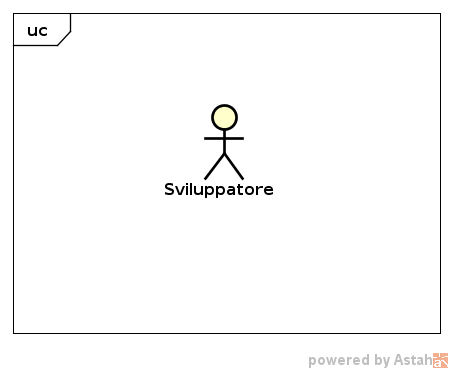
\includegraphics[scale=0.45]{img/solo_attori_sviluppatore.png}
   \caption{Diagramma per l'attore sviluppatore.}
\end{figure}


   \FloatBarrier
   \begin{figure}[ht]
   \centering
   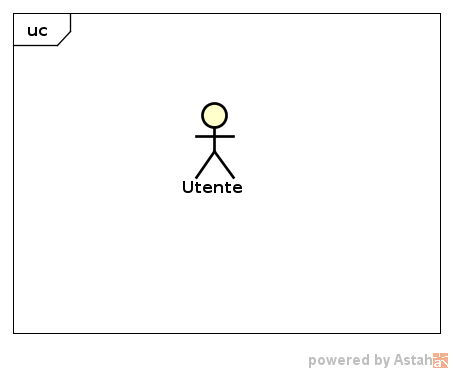
\includegraphics[scale=0.45]{img/solo_attori_utente.png}
   \caption{Diagramma per l'attore utente.}
\end{figure}

%\clearpage
\subsection{Contesto d'uso e funzionalità delle bolle}
\begin{itemize}
\item \textbf{Convertitore di valuta}\\
La bolla converte gli importi inseriti da una valuta all'altra. I tassi di cambio sono prelevati da una fonte esterna.
\item \textbf{Estrazione numeri casuali}\\
La bolla estrae un numero casualmente dal "range" impostato.
\item \textbf{Lista con checklist}\\
Il mittente inserisce gli elementi nella lista da inviare, ha inoltre a disposizione una lista di controllo (checklist) da cui prendere elementi. I riceventi possono spuntare elementi dalla lista ricevuta.
\item \textbf{Meteo}\\
 La bolla restituisce le previsioni meteo per la località scelta.
\item \textbf{Sondaggio}\\
Il mittente seleziona un certo numero di opzioni tra cui i riceventi possono scegliere.
\item \textbf{Traduttore automatico}\\
Una bolla che traduce il testo inserito nelle lingue selezionate.
\end{itemize}

\subsubsection{Caratteristiche degli utenti}
I prodotti realizzati con l'SDK, ovvero le bolle, sono rivolti agli
utenti di Rocket.chat.





\clearpage
%%%%%%%%%%%%%%%%%%%%%%%%%%%%%%%%%%%%%%%%%%%%%%%%%%%%%%%%%%%%%%%%%%%%%%%%%%%%%%%%%%
\section{Casi d'uso}
   \FloatBarrier
   \begin{figure}[ht]
   \centering
   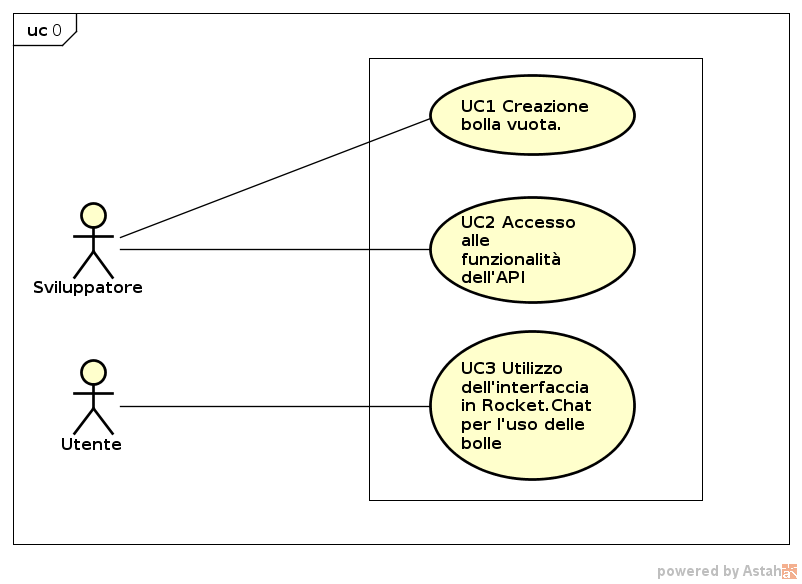
\includegraphics[scale=0.45]{img/0.png}
   \caption{Visione generale dei casi d'uso}
\end{figure}
\FloatBarrier
\subsection{Caso d'uso UC1: Creazione bolla vuota.}
\begin{itemize}
\item[]\textbf{Descrizione:} Lo sviluppatore sceglie di creare una nuova bolla. Il sistema inizializza una bolla vuota e predispone l'ambiente di lavoro (files di progetto pronti alle modifiche). La parte grafica della bolla include solo un contenitore vuoto d'ora in poi riferito come contenitore principale.
\item[]\textbf{Attori:} Sviluppatore. 
\item[]\textbf{Precondizione:} Il sistema è installato e pronto all'uso. 
\item[]\textbf{Postcondizione:} La bolla vuota è stata creata. 
\item[]\textbf{Scenario:}
 Lo sviluppatore sceglie di eseguire la procedura di inizializzazione per una nuova bolla e il sistema crea i files necessari.

 
\end{itemize}

\clearpage

\subsection{Caso d'uso UC2: Accesso alle funzionalità dell'API.}
\begin{itemize}
   \FloatBarrier
   \begin{figure}[ht]
   \centering
   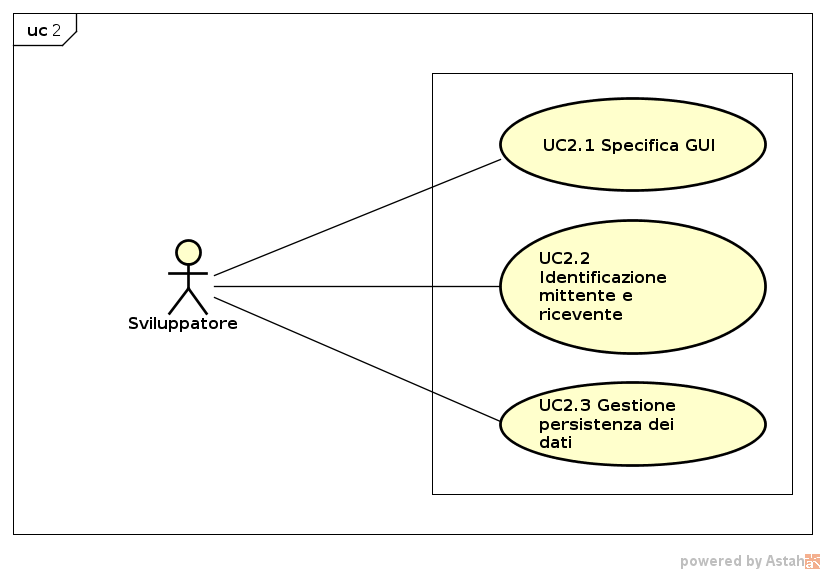
\includegraphics[scale=0.45]{img/2.png}
   \caption{Diagramma per il caso d'uso UC2.}
\end{figure}
\FloatBarrier
\item[]\textbf{Descrizione:} Lo sviluppatore utilizza le funzionalità offerte dall'API nella propria bolla.
\item[]\textbf{Attori:} Sviluppatore. 
\item[]\textbf{Precondizione:} Esiste una bolla (vuota o meno). 
\item[]\textbf{Postcondizione:} Lo sviluppatore ha aggiunto alla bolla le funzionalità desiderate. 
\item[]\textbf{Scenario:}
\begin{enumerate}
\item Lo sviluppatore utilizza le funzionalità per determinare la GUI (UC2.1).
\item Lo sviluppatore identifica le tipologie di utente (UC2.2).
\item Lo sviluppatore gestisce la persistenza dei dati (UC2.3). 
\end{enumerate} 
\end{itemize}

\clearpage

\subsection{Caso d'uso UC2.1: Specifica Gui.}
\begin{itemize}
   \FloatBarrier
   \begin{figure}[ht]
   \centering
   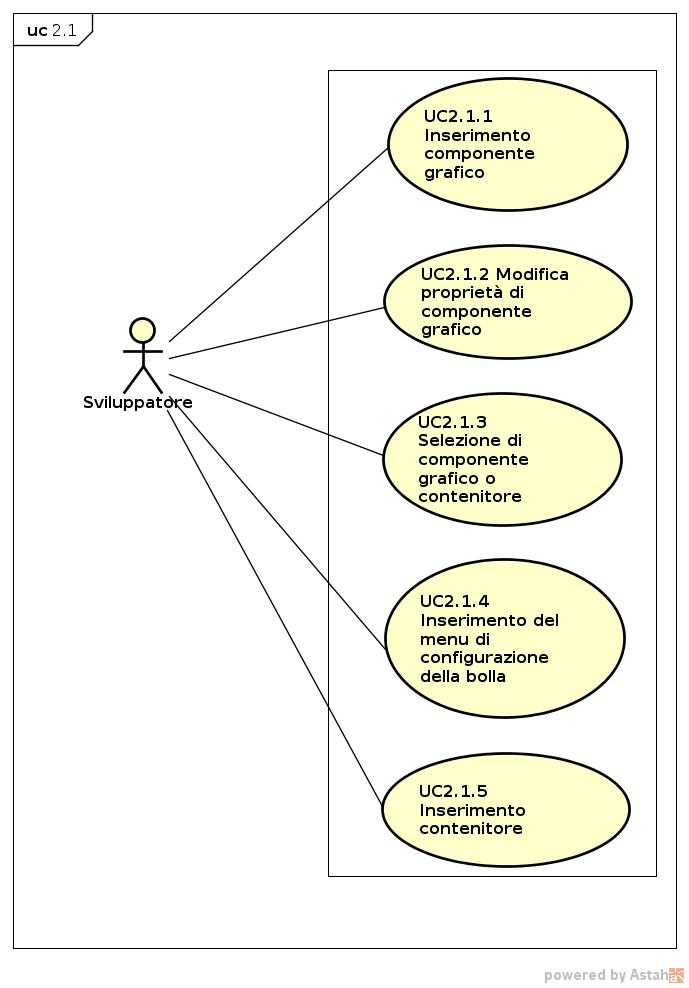
\includegraphics[scale=0.45]{img/2_1.png}
   \caption{Diagramma per il caso d'uso UC2.1.}
\end{figure}
\FloatBarrier
\item[]\textbf{Descrizione:} Lo sviluppatore utilizza le funzionalità offerte dall'API per descrivere l'aspetto visuale della bolla.
\item[]\textbf{Attori:} Sviluppatore. 
\item[]\textbf{Precondizione:} Esiste una bolla. 
\item[]\textbf{Postcondizione:} L'aspetto visuale della bolla è stato modificato. 
\item[]\textbf{Scenario:}
\begin{enumerate}
\item Lo sviluppatore inserisce un componente grafico (UC2.1.1).
\item Lo sviluppatore modifica le proprietà di un componente grafico (UC2.1.2).
\item Lo sviluppatore seleziona un componente grafico o un contenitore (UC2.1.3).
\item Lo sviluppatore inserisce il menu di configurazione della bolla (UC2.1.4)
\item Lo sviluppatore inserisce un contenitore (UC2.1.5)
\end{enumerate}
 
\end{itemize}

\subsection{Caso d'uso UC2.1.1: Inserimento di un componente grafico.}
\begin{itemize}
\item[]\textbf{Descrizione:} Lo sviluppatore inserisce un elemento grafico in un contenitore selezionato.
\item[]\textbf{Attori:} Sviluppatore. 
\item[]\textbf{Precondizione:} La bolla esiste e include almeno un contenitore. \'E stato selezionato il contenitore in cui inserire l'elemento. 
\item[]\textbf{Postcondizione:} Alla bolla è stato aggiunto un componente grafico nel contenitore selezionato. 
\item[]\textbf{Scenario:}
 Lo sviluppatore può inserire un componente grafico tra quelli supportati: \begin{itemize}
\item Componente immagine.
\item Componente campo di inserimento testo.
\item Componente pulsante.
\item Componente checkbox.
\item Componente radio button. 
\item Componente combobox
\end{itemize} 
\'E inoltre possibile inserire elementi realizzati dallo sviluppatore. 
\end{itemize}

\clearpage

\subsection{Caso d'uso UC2.1.2: Modifica proprietà di un componente grafico.}
\begin{itemize}
   \FloatBarrier
   \begin{figure}[ht]
   \centering
   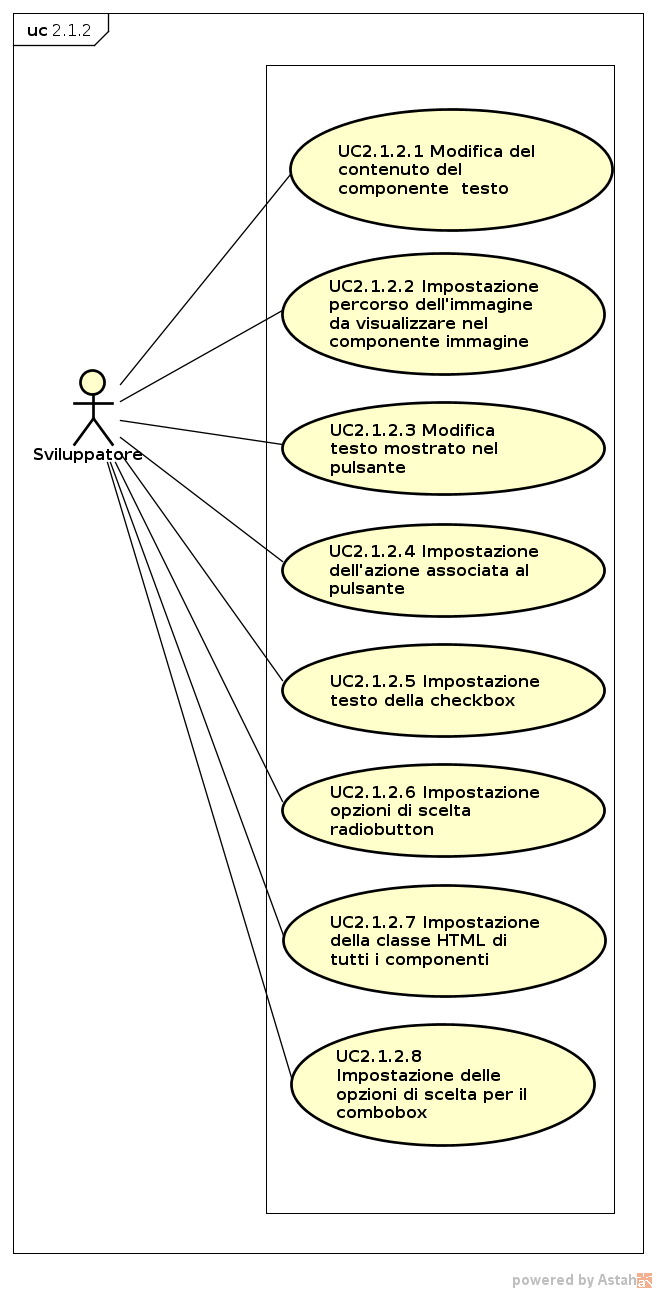
\includegraphics[scale=0.45]{img/2_1_2.png}
   \caption{Diagramma per il caso d'uso UC2.1.2.}
\end{figure}
\FloatBarrier
\item[]\textbf{Descrizione:} I componenti grafici hanno varie proprietà il cui valore può essere modificato. Alcune proprietà riguardano tutte le tipologie di componente grafico, altre sono valide solo per alcune. Una volta selezionato il componente grafico desiderato l'API permette di modificare il valore di una sua proprietà.
\item[]\textbf{Attori:} Sviluppatore. 
\item[]\textbf{Precondizione:} \'E stato selezionato un componente grafico. 
\item[]\textbf{Postcondizione:} \'E stata modificata una proprietà del componente grafico. 
\item[]\textbf{Scenario:}
 Dopo che l'elemento grafico è stato selezionato (uc2.1.3) lo sviluppatore può alterare le sue proprietà:

\begin{enumerate}
\item Modifica del contenuto dell'elemento di testo (UC2.1.2.1).
\item Selezione dell'immagine da visualizzare nell'elemento immagine (UC2.1.2.2).
\item Modifica testo mostrato nel pulsante (UC2.1.2.3).
\item Impostazione dell'azione associata al pulsante (UC2.1.2.4).
\item Impostazione testo della checkbox (UC2.1.2.5).
\item Impostazione opzioni di scelta radiobutton (UC2.1.2.6).
\item Impostazione classe HTML (UC2.1.2.7).
\item Impostazione opzioni di scelta combobox (UC2.1.2.7).
\end{enumerate} 
\end{itemize}

\subsection{Caso d'uso UC2.1.2.1: Modifica contenuto del componente testo.}
\begin{itemize}
\item[]\textbf{Descrizione:} Viene modificato il contenuto del componente di testo selezionato.
\item[]\textbf{Attori:} Sviluppatore. 
\item[]\textbf{Precondizione:} \'E stato selezionato il componente di tipo testo da modificare. 
\item[]\textbf{Postcondizione:} Il contenuto del componente testo è stato modificato. 
\item[]\textbf{Scenario:}
 Lo sviluppatore modifica il contenuto del componente di testo precedentemente selezionato. 
\end{itemize}

\subsection{Caso d'uso UC2.1.2.2: Impostazione percorso dell'immagine da visualizzare nel componente immagine.}
\begin{itemize}
\item[]\textbf{Descrizione:} Impostazione percorso dell'immagine da visualizzare nel componente immagine.
\item[]\textbf{Attori:} Sviluppatore. 
\item[]\textbf{Precondizione:} \'E stato selezionato un componente di tipo immagine. 
\item[]\textbf{Postcondizione:} \'E stata impostata la sorgente dell'immagine da visualizzare. 
\item[]\textbf{Scenario:}
 Lo sviluppatore imposta il percorso dell'immagine da visualizzare. 
\end{itemize}

\subsection{Caso d'uso UC2.1.2.3: Modifica testo mostrato nel pulsante.}
\begin{itemize}
\item[]\textbf{Descrizione:} Viene modificato il testo mostrato all'interno di un componente pulsante precedentemente selezionato.
\item[]\textbf{Attori:} Sviluppatore. 
\item[]\textbf{Precondizione:} \'E stato selezionato un componente di tipo pulsante. 
\item[]\textbf{Postcondizione:} Il testo mostrato nel pulsante è stato modificato. 
\item[]\textbf{Scenario:}
Lo sviluppatore modifica il testo mostrato all'interno di un pulsante. 
\end{itemize}

\subsection{Caso d'uso UC2.1.2.4: Impostazione dell'azione associata al pulsante.}
\begin{itemize}
\item[]\textbf{Descrizione:} Viene impostata l'azione che il sistema deve eseguire quando l'utente preme il pulsante.
\item[]\textbf{Attori:} Sviluppatore. 
\item[]\textbf{Precondizione:} \'E stato selezionato un componente di tipo pulsante. 
\item[]\textbf{Postcondizione:} L'azione associata al pulsante è stata impostata. 
\item[]\textbf{Scenario:}
Lo sviluppatore imposta l'azione che il sistema deve intraprendere quando l'utente preme il pulsante selezionato. 
\end{itemize}

\subsection{Caso d'uso UC2.1.2.5: Impostazione testo della checkbox.}
\begin{itemize}
\item[]\textbf{Descrizione:} Viene definito il testo da mostrare il corrispondenza di un componente checkbox.
\item[]\textbf{Attori:} Sviluppatore. 
\item[]\textbf{Precondizione:} \'E stato selezionato un componente di tipo checkbox. 
\item[]\textbf{Postcondizione:} \'E stato impostato il testo da visualizzane nel componente checkbox selezionato. 
\item[]\textbf{Scenario:}
 Lo sviluppatore imposta il testo da visualizzare insieme al componente di tipo checkbox 
\end{itemize}

\subsection{Caso d'uso UC2.1.2.6: Impostazione opzioni di scelta del radiobutton.}
\begin{itemize}
\item[]\textbf{Descrizione:} Vengono impostate le opzioni tra cui è possibile scegliere in un radiobutton.
\item[]\textbf{Attori:} Sviluppatore. 
\item[]\textbf{Precondizione:} \'E stato selezionato un componente di tipo radiobutton. 
\item[]\textbf{Postcondizione:} Sono state impostate le possibili opzioni tra cui l'utente può scegliere interagendo con il radiobutton selezionato. 
\item[]\textbf{Scenario:}
Lo sviluppatore imposta le possibili scelte offerte dal radiobutton precedentemente selezionato. 
\end{itemize}

\subsection{Caso d'uso UC2.1.2.7: Impostazione della classe HTML di tutti i componenti.}
\begin{itemize}
\item[]\textbf{Descrizione:} Per ciascun componente fornito dall'SDK è possibile specificare una o più classi HTML.
\item[]\textbf{Attori:} Sviluppatore. 
\item[]\textbf{Precondizione:} \'E stato selezionato un componente tra quelli forniti. 
\item[]\textbf{Postcondizione:} \'E stata specificata almeno una classe per il componente. 
\item[]\textbf{Scenario:}
Lo sviluppatore specifica la classe HTML per il componente selezionato 
\end{itemize}

\subsection{Caso d'uso UC2.1.2.8: Impostazione delle opzioni di scelta per il combobox.}
\begin{itemize}
\item[]\textbf{Descrizione:} Vengono impostate le opzioni tra cui l'utente dovrà scegliere utilizzando il combobox.
\item[]\textbf{Attori:} Sviluppatore. 
\item[]\textbf{Precondizione:} \'E stato selezionato un elemento di tipo combobox. 
\item[]\textbf{Postcondizione:} Sono state impostate le opzioni tra cui scegliere nel combobox. 
\item[]\textbf{Scenario:}
Lo sviluppatore specifica le opzioni tra cui scegliere nel combobox 
\end{itemize}

\subsection{Caso d'uso UC2.1.3: Selezione di un componente grafico o di un contenitore.}
\begin{itemize}
\item[]\textbf{Descrizione:} Viene selezionato un componente grafico o un contenitore.
\item[]\textbf{Attori:} Sviluppatore. 
\item[]\textbf{Precondizione:} La bolla è stata creata. 
\item[]\textbf{Postcondizione:} \'E stato selezionato un componente grafico o un contenitore. 
\item[]\textbf{Scenario:}
 Lo sviluppatore seleziona un componente grafico. 
\end{itemize}

\subsection{Caso d'uso UC2.1.4: Inserimento del menu di configurazione della bolla.}
\begin{itemize}
\item[]\textbf{Descrizione:} Viene definito il menu per configurare la bolla del tipo selezionato.
\item[]\textbf{Attori:} Sviluppatore. 
\item[]\textbf{Precondizione:} \'E stato definito un nuovo tipo di bolla. 
\item[]\textbf{Postcondizione:} \'E stato definito il menu di configurazione per l'invio di una bolla del tipo corrente. 
\item[]\textbf{Scenario:}
Lo sviluppatore definisce il menu di configurazione per l'invio della bolla del tipo corrente. 
\end{itemize}

\subsection{Caso d'uso UC2.1.5: Inserimento contenitore.}
\begin{itemize}
\item[]\textbf{Descrizione:} Lo sviluppatore inserisce  un contenitore in un contenitore selezionato.
\item[]\textbf{Attori:} Sviluppatore. 
\item[]\textbf{Precondizione:} La bolla esiste e include almeno un contenitore. \'E stato
selezionato il contenitore in cui inserire il contenitore. 
\item[]\textbf{Postcondizione:} Alla bolla è stato aggiunto un
contenitore nel contenitore selezionato. 
\item[]\textbf{Scenario:}
Lo sviluppatore può inserire un contenitore nel contenitore selezionato. 
\end{itemize}

\subsection{Caso d'uso UC2.2: Identificazione Mittente o Ricevente.}
\begin{itemize}
\item[]\textbf{Descrizione:} Ciascuna istanza di bolla viene creata da un utente e poi inviata ad uno o più altri utenti. Generalmente ci si aspetta che la bolla si comporti diversamente nelle due situazioni, per esempio fornendo una procedura di inizializzazione al mittente. \'E dunque possibile descrivere un comportamento diverso per il mittente e per il ricevente della bolla.
\item[]\textbf{Attori:} Sviluppatore. 
\item[]\textbf{Precondizione:} La bolla esiste. 
\item[]\textbf{Postcondizione:} Sono stati distinti mittente e ricevente. 
\item[]\textbf{Scenario:}
Lo sviluppatore utilizza la funzionalità che permette di identificare a runtime se la bolla è visualizzata dal mittente o da altri utenti. 
\end{itemize}

\clearpage

\subsection{Caso d'uso UC2.3: Gestione persistenza dei dati.}
\begin{itemize}
   \FloatBarrier
   \begin{figure}[ht]
   \centering
   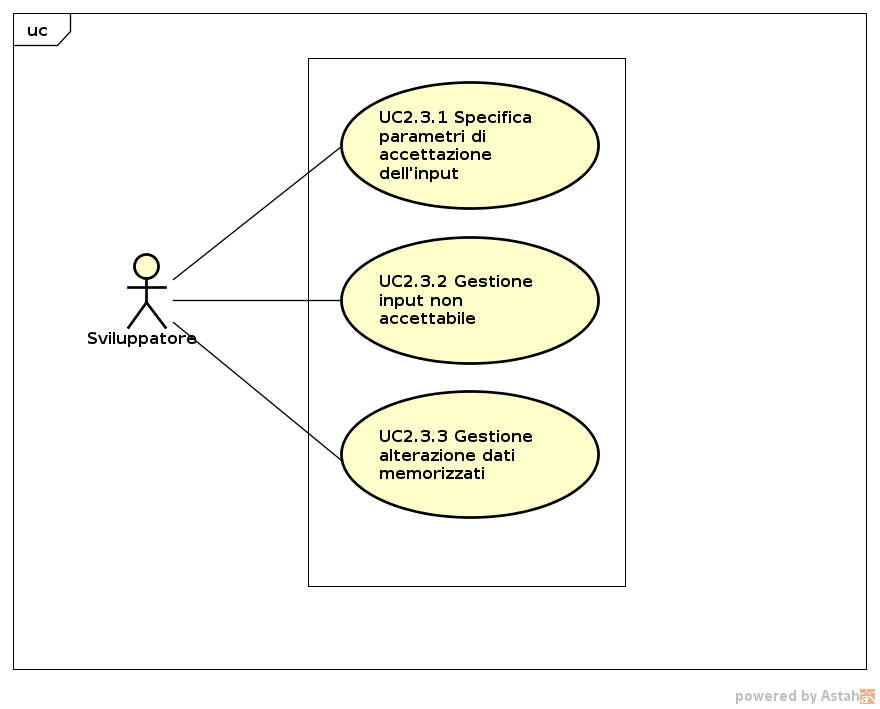
\includegraphics[scale=0.45]{img/2_3.png}
   \caption{Diagramma per il caso d'uso UC2.3.}
\end{figure}
\FloatBarrier
\item[]\textbf{Descrizione:} Viene offerta un'interfaccia al sistema di memorizzazione dei dati che fornisca in modo trasparente funzionalità utili allo sviluppo delle bolle. In particolare il sistema distingue automaticamente i dati relativi alla singola istanza di bolla.
\item[]\textbf{Attori:} Sviluppatore. 
\item[]\textbf{Precondizione:} La bolla esiste. 
\item[]\textbf{Postcondizione:} \'E stata impostata la persistenza di un'informazione. 
\item[]\textbf{Scenario:}
\begin{enumerate}

\item Lo sviluppatore specifica i parametri di accettazione dell'input (UC2.3.1)
\item Lo sviluppatore specifica come gestire l'input non accettabile (UC2.3.2) 
\item Lo sviluppatore specifica come gestire l'alterazione dei dati memorizzati (UC2.3.3)
\end{enumerate} 
\end{itemize}

\subsection{Caso d'uso UC2.3.1: Specifica parametri di accettazione dell'input.}
\begin{itemize}
\item[]\textbf{Descrizione:} Vengono specificate le possibili forme che l'input deve assumere. Vengono definiti i controlli da effettuare sui dati immessi dagli utenti.
\item[]\textbf{Attori:} Sviluppatore. 
\item[]\textbf{Precondizione:} La bolla esiste. 
\item[]\textbf{Postcondizione:} Sono stati specificati i controlli da effettuare sull'input. 
\item[]\textbf{Scenario:}
Lo sviluppatore specifica i controlli da eseguire sull'input 
\end{itemize}

\clearpage

\subsection{Caso d'uso UC2.3.2: Gestione input non accettabile.}
\begin{itemize}
   \FloatBarrier
   \begin{figure}[ht]
   \centering
   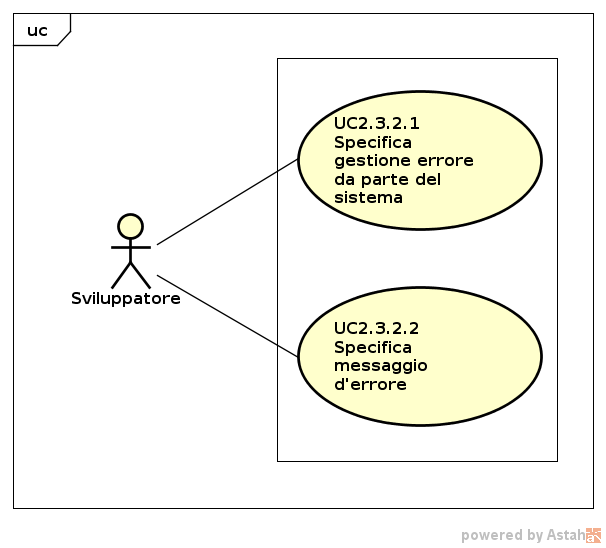
\includegraphics[scale=0.45]{img/2_3_2.png}
   \caption{Diagramma per il caso d'uso UC2.3.2.}
\end{figure}
\FloatBarrier
\item[]\textbf{Descrizione:} Viene gestito l'input rifiutato dai controlli e vengono specificate le azioni da intraprendere.
\item[]\textbf{Attori:} Sviluppatore. 
\item[]\textbf{Precondizione:} Sono stati specificati i parametri di accettazione dell'input (UC2.3.1). 
\item[]\textbf{Postcondizione:} \'E stato specificato come gestire l'input non accettabile. 
\item[]\textbf{Scenario:}
\begin{enumerate}

\item Lo sviluppatore specifica come il sistema deve gestire gli errori nell'input (UC2.3.2.1)
\item Lo sviluppatore specifica il messaggio d'errore che l'utente deve visualizzare (UC2.3.2.2)

\end{enumerate} 
\end{itemize}

\subsection{Caso d'uso UC2.3.2.1: Specifica gestione errore da parte del sistema.}
\begin{itemize}
\item[]\textbf{Descrizione:} Viene specificato come il sistema deve gestire gli errori nell'input.
\item[]\textbf{Attori:} Sviluppatore. 
\item[]\textbf{Precondizione:} Sono stati specificati i parametri di accettazione dell'input (UC2.3.1). 
\item[]\textbf{Postcondizione:} \'E stato specificato come il sistema deve gestire gli errori nell'input. 
\item[]\textbf{Scenario:}
Lo sviluppatore specifica come il sistema deve gestire gli errori nell'input 
\end{itemize}

\subsection{Caso d'uso UC2.3.2.2: Specifica messaggio di errore.}
\begin{itemize}
\item[]\textbf{Descrizione:} Viene specificato il messaggio d'errore che l'utente deve visualizzare.
\item[]\textbf{Attori:} Sviluppatore. 
\item[]\textbf{Precondizione:} Sono stati specificati i parametri di accettazione dell'input (UC2.3.1). 
\item[]\textbf{Postcondizione:} \'E stato specificato il messaggio d'errore per l'utente. 
\item[]\textbf{Scenario:}
Lo sviluppatore specifica il messaggio di errore per l'utente 
\end{itemize}

\subsection{Caso d'uso UC2.3.3: Gestione dati memorizzati.}
\begin{itemize}
\item[]\textbf{Descrizione:} Viene gestita l'alterazione (aggiunta,modifica,rimozione) dei dati memorizzati.
\item[]\textbf{Attori:} Sviluppatore. 
\item[]\textbf{Precondizione:} Sono stati specificati i parametri di accettazione dell'input (UC2.3.1). 
\item[]\textbf{Postcondizione:} \'E stato specificato come gestire l'alterazione dei dati memorizzati. 
\item[]\textbf{Scenario:}
Lo sviluppatore specifica come gestire l'alterazione dei dati memorizzati 
\end{itemize}

\clearpage

\subsection{Caso d'uso UC3: Utilizzo dell'interfaccia in Rocket.Chat per l'uso delle bolle.}
\begin{itemize}
   \FloatBarrier
   \begin{figure}[ht]
   \centering
   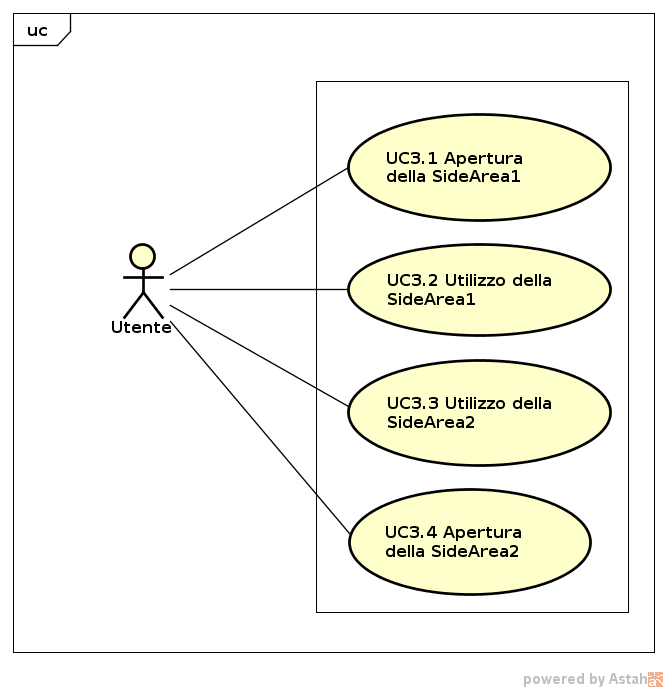
\includegraphics[scale=0.45]{img/3.png}
   \caption{Diagramma per il caso d'uso UC3.}
\end{figure}
\FloatBarrier
\item[]\textbf{Descrizione:} Viene fornita una modifica all'interfaccia di Rocket.Chat. In particolare vengono aggiunti due pulsanti alla tabbar di Rocket.Chat. Questi permettono di aprire le SideAreas che permettono la creazione e la visualizzazione delle bolle.
\item[]\textbf{Attori:} Utente. 
\item[]\textbf{Precondizione:} Il sistema è installato e pronto all'uso. 
\item[]\textbf{Postcondizione:} \'E stato possibile utilizzare le funzionalità offerte. 
\item[]\textbf{Scenario:}
\begin{enumerate}
\item Apertura della SideArea1(UC3.1)
\item Utilizzo della SideArea1 (UC3.2)
\item Utilizzo della SideArea2 (UC3.3)
\item Apertura della SideArea2 (UC3.4)
\end{enumerate} 
\end{itemize}

\subsection{Caso d'uso UC3.1: Apertura della SideArea1.}
\begin{itemize}
\item[]\textbf{Descrizione:} Attraverso la pressione del primo dei pulsanti aggiunti alla tabbar di Rocket.Chat è possibile accedere alla SideArea1.
\item[]\textbf{Attori:} Utente. 
\item[]\textbf{Precondizione:} Il sistema è installato e pronto all'uso. 
\item[]\textbf{Postcondizione:} \'E avvenuta l'apertura della SideArea1. 
\item[]\textbf{Scenario:}
L'utente preme il primo dei pulsanti nella tabbar di Rocket.Chat e viene aperta la SideArea1 
\end{itemize}

\clearpage

\subsection{Caso d'uso UC3.2: Utilizzo della SideArea1.}
\begin{itemize}
   \FloatBarrier
   \begin{figure}[ht]
   \centering
   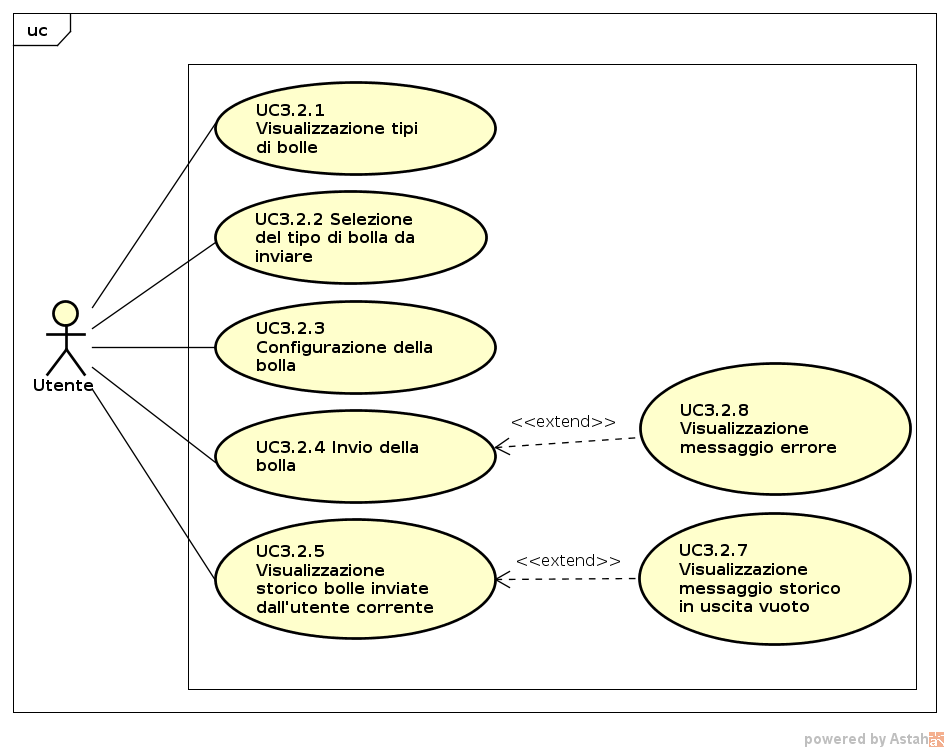
\includegraphics[scale=0.45]{img/3_2.png}
   \caption{Diagramma per il caso d'uso UC3.2.}
\end{figure}
\FloatBarrier
\item[]\textbf{Descrizione:} Viene usata la SideArea1.
\item[]\textbf{Attori:} Utente. 
\item[]\textbf{Precondizione:} \'E stata aperta la SideArea1 (UC3.1). 
\item[]\textbf{Postcondizione:} \'E stata utilizzata la SideArea1. 
\item[]\textbf{Scenario:}
\begin{enumerate}
\item L'utente visualizza i tipi di bolla disponibili (UC3.2.1)
\item L'utente seleziona il tipo di bolla da inviare (UC3.2.2)
\item L'utente configura la bolla (UC3.2.3)
\item L'utente invia la bolla (UC3.2.4)
\item L'utente visualizza lo storico delle bolle inviate (UC3.2.5)
\end{enumerate} 
\end{itemize}

\subsection{Caso d'uso UC3.2.1: Visualizzazione tipi di bolle.}
\begin{itemize}
\item[]\textbf{Descrizione:} Vengono visualizzati i tipi di bolla presenti nel sistema.
\item[]\textbf{Attori:} Utente. 
\item[]\textbf{Precondizione:} \'E stata aperta la SideArea1 (UC3.1). 
\item[]\textbf{Postcondizione:} Sono stati visualizzati i tipi di bolla presenti. 
\item[]\textbf{Scenario:}
L'utente visualizza i tipi di bolla presenti nel sistema. 
\end{itemize}

\subsection{Caso d'uso UC3.2.2: Selezione del tipo di bolla da inviare.}
\begin{itemize}
\item[]\textbf{Descrizione:} Viene selezionato il tipo di bolla da inviare.
\item[]\textbf{Attori:} Utente. 
\item[]\textbf{Precondizione:} Sono stati visualizzati i tipi di bolla presenti nel sistema (UC3.2.1). 
\item[]\textbf{Postcondizione:} \'E stato selezionato il tipo di bolla da inviare. 
\item[]\textbf{Scenario:}
L'utente ha selezionato il tipo di bolla da inviare. 
\end{itemize}

\subsection{Caso d'uso UC3.2.3: Configurazione della bolla.}
\begin{itemize}
\item[]\textbf{Descrizione:} Viene configurata la bolla da inviare utilizzando l'apposito menu di configurazione (UC2.1.4).
\item[]\textbf{Attori:} Utente. 
\item[]\textbf{Precondizione:} \'E stata selezionata la bolla da inviare (UC3.2.2). 
\item[]\textbf{Postcondizione:} La bolla è stata configurata per l'invio. 
\item[]\textbf{Scenario:}
L'utente configura la bolla utilizzando il menu apposito. 
\end{itemize}

\subsection{Caso d'uso UC3.2.4: Invio della bolla.}
\begin{itemize}
\item[]\textbf{Descrizione:} Viene inviata la bolla.
\item[]\textbf{Attori:} Utente. 
\item[]\textbf{Precondizione:} La bolla è stata configurata (UC3.2.3). 
\item[]\textbf{Postcondizione:} La bolla è stata inviata. 
\item[]\textbf{Scenario:}
L'utente invia la bolla. 
\item[]\textbf{Estensioni:}
Viene visualizzato un messaggio di errore quando i dati inseriti nella configurazione non sono corretti (UC3.2.8) 
\end{itemize}

\subsection{Caso d'uso UC3.2.5: Visualizzazione storico bolle inviate dall'utente corrente.}
\begin{itemize}
\item[]\textbf{Descrizione:} Vengono visualizzate le bolle inviate dall'utente corrente.
\item[]\textbf{Attori:} Utente. 
\item[]\textbf{Precondizione:} La SideArea1 è stata acceduta (UC3.1). 
\item[]\textbf{Postcondizione:} \'E stato visualizzato lo storico delle bolle inviate. 
\item[]\textbf{Scenario:}
L'utente visualizza lo storico delle bolle inviate. 
\item[]\textbf{Estensioni:}
Viene visualizzato un messaggio quando lo storico non contiene bolle (UC3.2.7). 
\end{itemize}

\subsection{Caso d'uso UC3.2.7: Visualizzazione messaggio storico in uscita vuoto.}
\begin{itemize}
\item[]\textbf{Descrizione:} Viene visualizzato un messaggio che informa che lo storico delle bolle inviate è vuoto.
\item[]\textbf{Attori:} Utente. 
\item[]\textbf{Precondizione:} Lo storico delle bolle inviate è vuoto. 
\item[]\textbf{Postcondizione:} \'E stato visualizzato il messaggio che spiega che lo storico delle bolle inviate è vuoto. 
\item[]\textbf{Scenario:}
L'utente visualizza il messaggio che spiega che lo storico delle bolle inviate è vuoto. 
\end{itemize}

\subsection{Caso d'uso UC3.2.8: Visualizzazione messaggio errore.}
\begin{itemize}
\item[]\textbf{Descrizione:} Viene visualizzato un messaggio di errore nel caso in cui i dati inseriti nella configurazione non fossero corretti.
\item[]\textbf{Attori:} Utente. 
\item[]\textbf{Precondizione:} \'E stata configurata la bolla da inviare. 
\item[]\textbf{Postcondizione:} \'E stato visualizzato il messaggio di errore. 
\item[]\textbf{Scenario:}
L'utente visualizza il messaggio di errore 
\end{itemize}

\clearpage

\subsection{Caso d'uso UC3.3: Utilizzo della SideArea2.}
\begin{itemize}
   \FloatBarrier
   \begin{figure}[ht]
   \centering
   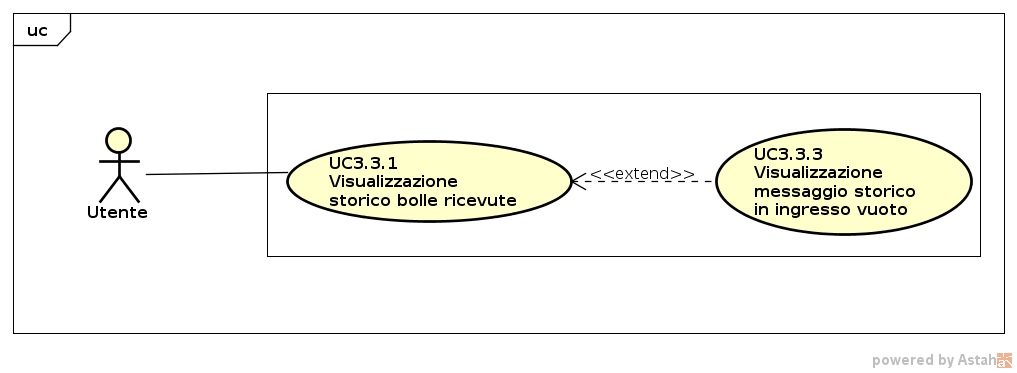
\includegraphics[scale=0.45]{img/3_3.png}
   \caption{Diagramma per il caso d'uso UC3.3.}
\end{figure}
\FloatBarrier
\item[]\textbf{Descrizione:} Viene usata la SideArea2.
\item[]\textbf{Attori:} Utente. 
\item[]\textbf{Precondizione:} \'E stata aperta la SideArea2. 
\item[]\textbf{Postcondizione:} \'E stata utilizzata la SideArea2. 
\item[]\textbf{Scenario:}
L'utente ha utilizzato la SideArea2. 
\end{itemize}

\subsection{Caso d'uso UC3.3.1: Visualizzazione storico bolle ricevute.}
\begin{itemize}
\item[]\textbf{Descrizione:} Viene visualizzato lo storico delle bolle ricevute.
\item[]\textbf{Attori:} Utente. 
\item[]\textbf{Precondizione:} La SideArea2 è stata acceduta (UC3.1). 
\item[]\textbf{Postcondizione:} \'E stato visualizzato lo storico delle bolle ricevute. 
\item[]\textbf{Scenario:}
L'utente visualizza lo storico delle bolle ricevute. 
\item[]\textbf{Estensioni:}
Viene visualizzato un messaggio quando lo storico non contiene bolle (UC3.3.3). 
\end{itemize}

\subsection{Caso d'uso UC3.3.3: Visualizzazione messaggio storico in ingresso vuoto.}
\begin{itemize}
\item[]\textbf{Descrizione:} Viene visualizzato un messaggio che informa che lo storico delle bolle ricevute è vuoto.
\item[]\textbf{Attori:} Utente. 
\item[]\textbf{Precondizione:} Lo storico delle bolle ricevute è vuoto. 
\item[]\textbf{Postcondizione:} \'E stato visualizzato il messaggio che spiega che lo storico delle bolle ricevute è vuoto. 
\item[]\textbf{Scenario:}
L'utente visualizza il messaggio che spiega che lo storico delle bolle ricevute è vuoto. 
\end{itemize}

\subsection{Caso d'uso UC3.4: Apertura della SideArea2.}
\begin{itemize}
\item[]\textbf{Descrizione:} Attraverso la pressione del secondo dei pulsanti aggiunti alla tabbar di Rocket.Chat è possibile accedere alla SideArea2.
\item[]\textbf{Attori:} Utente. 
\item[]\textbf{Precondizione:} Il sistema è installato e pronto all'uso. 
\item[]\textbf{Postcondizione:} \'E avvenuta l'apertura della SideArea2. 
\item[]\textbf{Scenario:}
L'utente preme il secondo dei pulsanti nella tabbar di Rocket.Chat e viene aperta la SideArea2 
\end{itemize}

\clearpage

\subsection{Caso d'uso UC0-cv: Bolla convertitore di valuta.}
\begin{itemize}
   \FloatBarrier
   \begin{figure}[ht]
   \centering
   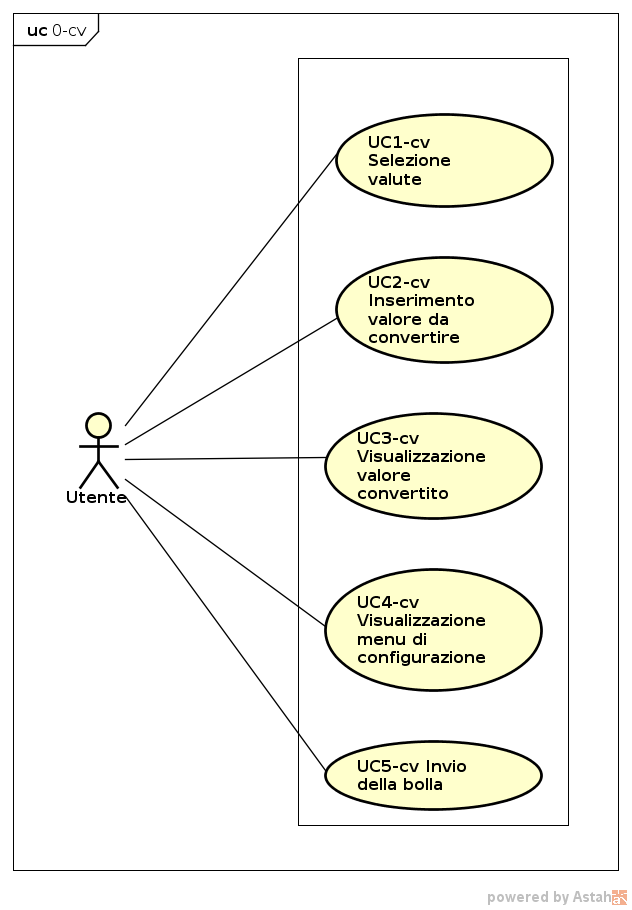
\includegraphics[scale=0.45]{img/soldi.png}
   \caption{Diagramma per il caso d'uso UC0-cv.}
\end{figure}
\FloatBarrier
\item[]\textbf{Descrizione:} La bolla converte gli importi inseriti da una valuta all'altra.
\item[]\textbf{Attori:} Utente. 
\item[]\textbf{Precondizione:} La bolla è utilizzabile sul sistema del mittente e del ricevente. 
\item[]\textbf{Postcondizione:} La bolla ha convertito l'importo nella valuta di destinazione. 
\item[]\textbf{Scenario:}
\begin{enumerate}



\item L'utente seleziona la valuta in ingresso e quella in uscita (UC1-cv)

\item L'utente seleziona un importo da convertire (UC2-cv).

\item Mittente e ricevente visualizzano l'importo convertito (UC3-cv).
\item L'utente visualizza il menu di configurazione della bolla (UC4-cv)
\item L'utente invia la bolla (UC5-cv)

\end{enumerate} 
\end{itemize}

\subsection{Caso d'uso UC1-cv: Seleziona valute.}
\begin{itemize}
\item[]\textbf{Descrizione:} L'utente seleziona la valuta di entrata e quelle di uscita.
\item[]\textbf{Attori:} Utente. 
\item[]\textbf{Precondizione:} \'E stato visualizzato il menu di configurazione (UC4-cv). 
\item[]\textbf{Postcondizione:} Le valute sono state selezionate. 
\item[]\textbf{Scenario:}
L'utente seleziona le valute tra cui effettuare la conversione 
\end{itemize}

\subsection{Caso d'uso UC2-cv: Inserimento importo da convertire.}
\begin{itemize}
\item[]\textbf{Descrizione:} Viene inserito l'importo da convertire.
\item[]\textbf{Attori:} Utente. 
\item[]\textbf{Precondizione:} \'E stato visualizzato il menu di configurazione (UC4-cv). 
\item[]\textbf{Postcondizione:} L'importo è stato inserito. 
\item[]\textbf{Scenario:}
L'utente inserisce l'importo da convertire. 
\end{itemize}

\subsection{Caso d'uso UC3-cv: Visualizzazione valore convertito.}
\begin{itemize}
\item[]\textbf{Descrizione:} Vengono visualizzati i valori convertiti.
\item[]\textbf{Attori:} Utente. 
\item[]\textbf{Precondizione:} La bolla è stata inviata (UC5-cv). 
\item[]\textbf{Postcondizione:} L'importo è stato convertito secondo i tassi di cambio richiesti. 
\item[]\textbf{Scenario:}
L'utente e il ricevente visualizzano i valori convertiti. 
\end{itemize}

\subsection{Caso d'uso UC4-cv: Visualizzazione menu di configurazione.}
\begin{itemize}
\item[]\textbf{Descrizione:} Viene visualizzato il menu di configurazione per la bolla convertitore di valuta.
\item[]\textbf{Attori:} Utente. 
\item[]\textbf{Precondizione:} La bolla è utilizzabile sul sistema del mittente e in quello del ricevente. 
\item[]\textbf{Postcondizione:} \'E stato visualizzato il menu di configurazione per la bolla convertitore di valuta. 
\item[]\textbf{Scenario:}
L'utente visualizza il menu di configurazione per la bolla convertitore di valuta 
\end{itemize}

\subsection{Caso d'uso UC5-cv: Invio della bolla.}
\begin{itemize}
\item[]\textbf{Descrizione:} La bolla convertitore di valuta viene inviata.
\item[]\textbf{Attori:} Utente. 
\item[]\textbf{Precondizione:} Sono state selezionate le valute in ingresso e in uscita (UC1-cv) ed è stato inserito l'importo da convertire (UC2-cv). 
\item[]\textbf{Postcondizione:} La bolla è stata inviata. 
\item[]\textbf{Scenario:}
L'utente deve poter inviare la bolla convertitore di valuta 
\end{itemize}

\clearpage

\subsection{Caso d'uso UC0-dd: Bolla estrazione numeri casuali.}
\begin{itemize}
   \FloatBarrier
   \begin{figure}[ht]
   \centering
   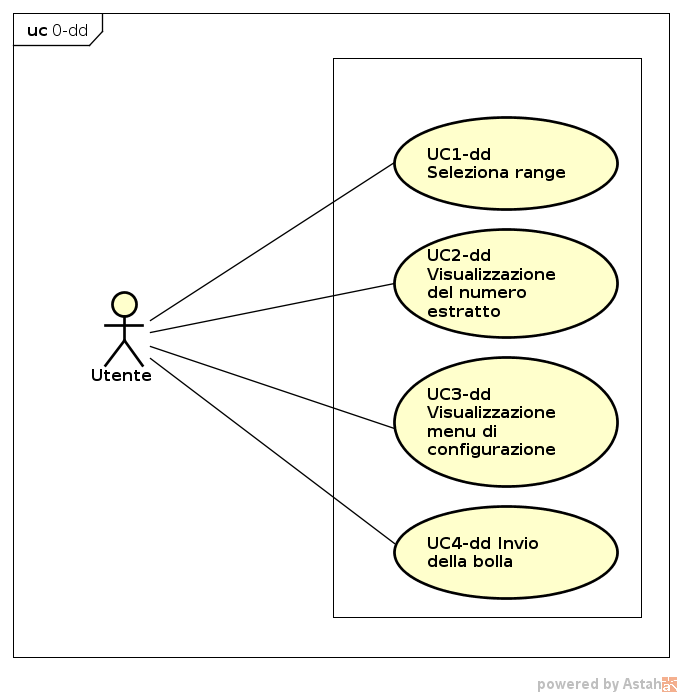
\includegraphics[scale=0.45]{img/random.png}
   \caption{Diagramma per il caso d'uso UC0-dd.}
\end{figure}
\FloatBarrier
\item[]\textbf{Descrizione:} Viene estratto un numero casuale da un range impostato.
\item[]\textbf{Attori:} Utente. 
\item[]\textbf{Precondizione:} La bolla è utilizzabile sul sistema del mittente e del ricevente. 
\item[]\textbf{Postcondizione:} \'E il stato visualizzato il numero estratto. 
\item[]\textbf{Scenario:}
\begin{enumerate}
\item L'utente seleziona il range da cui estrarre il numero casuale (UC1-dd)
\item L'utente e il ricevente visualizzano il numero estratto (UC2-dd)
\item L'utente visualizza il menu di configurazione della bolla (UC3-dd)
\item L'utente invia la bolla (UC4-dd)
\end{enumerate} 
\end{itemize}

\subsection{Caso d'uso UC1-dd: Seleziona range.}
\begin{itemize}
\item[]\textbf{Descrizione:} Viene selezionato il range da cui estrarre il numero casuale.
\item[]\textbf{Attori:} Utente. 
\item[]\textbf{Precondizione:} \'E stato visualizzato il menu di configurazione (UC3-dd). 
\item[]\textbf{Postcondizione:} Il range è stato impostato. 
\item[]\textbf{Scenario:}
L'utente seleziona il range da cui estrarre il numero 
\end{itemize}

\subsection{Caso d'uso UC2-dd: Visualizzazione numero estratto.}
\begin{itemize}
\item[]\textbf{Descrizione:} Viene visualizzato il numero estratto.
\item[]\textbf{Attori:} Utente. 
\item[]\textbf{Precondizione:} La bolla è stata inviata (UC4-dd). 
\item[]\textbf{Postcondizione:} Viene mostrato il numero estratto. 
\item[]\textbf{Scenario:}
L'utente e il ricevente visualizzano il numero estratto 
\end{itemize}

\subsection{Caso d'uso UC3-dd: Visualizzazione menu di configurazione.}
\begin{itemize}
\item[]\textbf{Descrizione:} Viene visualizzato il menu di configurazione per la bolla estrazione di numero casuale.
\item[]\textbf{Attori:} Utente. 
\item[]\textbf{Precondizione:} La bolla è utilizzabile sul sistema del mittente e su quello del ricevente. 
\item[]\textbf{Postcondizione:} \'E stato visualizzato il menu di configurazione per la bolla estrazione di numero casuale. 
\item[]\textbf{Scenario:}
L'utente visualizza il menu di configurazione per la bolla estrazione di numero casuale. 
\end{itemize}

\subsection{Caso d'uso UC4-dd: Invio della bolla.}
\begin{itemize}
\item[]\textbf{Descrizione:} Viene inviata la bolla estrazione di numero casuale.
\item[]\textbf{Attori:} Utente. 
\item[]\textbf{Precondizione:} \'E stato selezionato il range (UC1-dd). 
\item[]\textbf{Postcondizione:} La bolla è stata inviata. 
\item[]\textbf{Scenario:}
L'utente invia la bolla estrazione di numero casuale 
\end{itemize}

\clearpage

\subsection{Caso d'uso UC0-ls: Lista con checklist.}
\begin{itemize}
   \FloatBarrier
   \begin{figure}[ht]
   \centering
   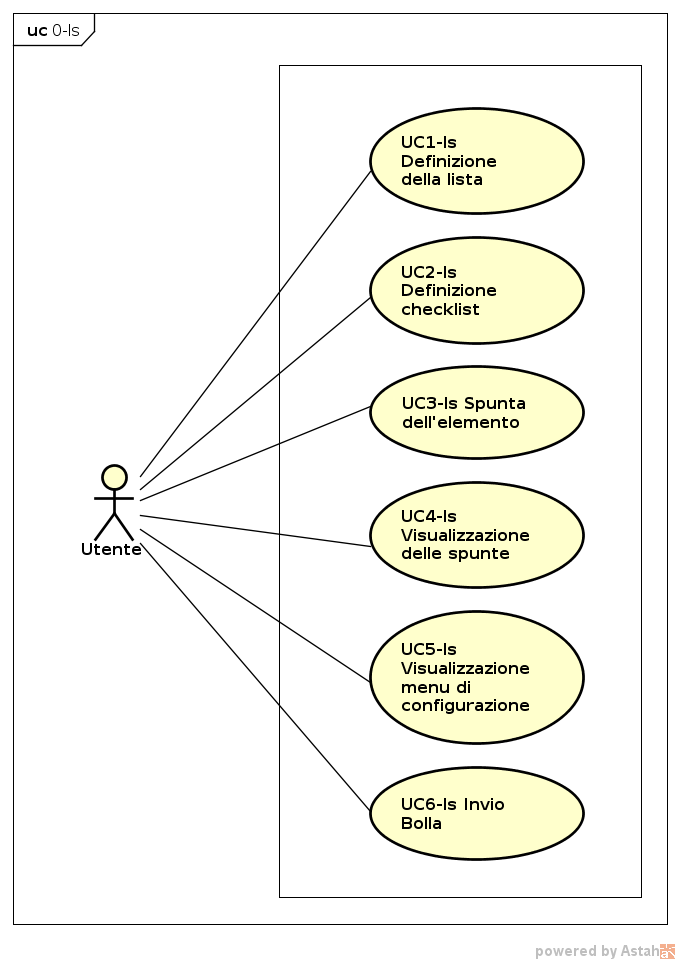
\includegraphics[scale=0.45]{img/lista0.png}
   \caption{Diagramma per il caso d'uso UC0-ls.}
\end{figure}
\FloatBarrier
\item[]\textbf{Descrizione:} L'utente inserisce gli elementi nella lista da inviare, ha inoltre a disposizione una lista di controllo (checklist) da cui prendere elementi. I riceventi possono spuntare elementi dalla lista ricevuta.
\item[]\textbf{Attori:} Utente. 
\item[]\textbf{Precondizione:} La bolla è utilizzabile sul sistema del mittente e del ricevente. 
\item[]\textbf{Postcondizione:} L'utente ha composto e inviato la lista e i riceventi hanno potuto spuntare delle voci. 
\item[]\textbf{Scenario:}
\begin{enumerate}



\item L'utente definisce la lista da inviare (UC1-ls)

\item L'utente definisce delle checklist predefinite a cui attingere per formare la lista da inviare (UC2-ls).

\item Il ricevente spunta una voce della lista che gli è stata inviata (UC3-ls).

\item L'utente visualizza le spunte effettuate (UC4-ls)

\item L'utente visualizza il menu di configurazione della bolla (UC5-ls)
\item L'utente invia la bolla (UC6-ls)


\end{enumerate} 
\end{itemize}

\clearpage

\subsection{Caso d'uso UC1-ls: Definizione della lista.}
\begin{itemize}
   \FloatBarrier
   \begin{figure}[ht]
   \centering
   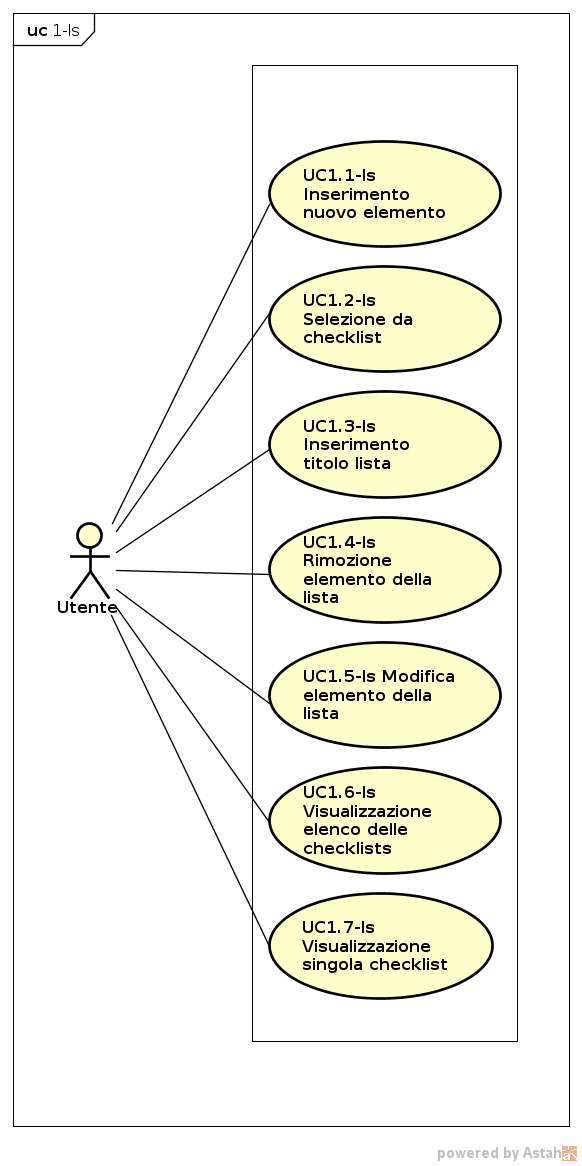
\includegraphics[scale=0.45]{img/lista1.png}
   \caption{Diagramma per il caso d'uso UC1-ls.}
\end{figure}
\FloatBarrier
\item[]\textbf{Descrizione:} L'utente definisce una lista da inviare.
\item[]\textbf{Attori:} Utente. 
\item[]\textbf{Precondizione:} \'E stato visualizzato il menu di configurazione (UC5-ls). 
\item[]\textbf{Postcondizione:} La lista è pronta per essere inviata. 
\item[]\textbf{Scenario:}
\begin{enumerate}



\item L'utente inserisce un elemento nella lista (UC1.1-ls).

\item L'utente inserisce un elemento nella lista scegliendolo dalla checklist definita in precedenza (UC1.2-ls).
\item L'utente inserisce un titolo per la lista (UC1.3-ls)
\item L'utente rimuove un elemento dalla lista (UC1.4-ls)
\item L'utente modifica un elemento della lista (UC1.5-ls)
\item L'utente visualizza l'elenco delle checklist (UC1.6-ls)
\item L'utente visualizza una singola checklist (UC1.7-ls)

\end{enumerate} 
\end{itemize}

\subsection{Caso d'uso UC1.1-ls: Inserimento di un nuovo elemento.}
\begin{itemize}
\item[]\textbf{Descrizione:} L'utente inserisce manualmente un nuovo elemento.
\item[]\textbf{Attori:} Utente. 
\item[]\textbf{Precondizione:} \'E stato visualizzato il menu di configurazione (UC5-ls). 
\item[]\textbf{Postcondizione:} Una voce è stata inserita nella lista. 
\item[]\textbf{Scenario:}
L'utente inserisce un elemento nella lista da inviare. 
\end{itemize}

\subsection{Caso d'uso UC1.2-ls: Selezione della voce da checklist.}
\begin{itemize}
\item[]\textbf{Descrizione:} Viene selezionata un voce da una delle checklist da inserire nella lista da inviare.
\item[]\textbf{Attori:} Utente. 
\item[]\textbf{Precondizione:} \'E stata visualizzata la singola checklist che contiene l'elemento da aggiungere (UC1.7-ls). 
\item[]\textbf{Postcondizione:} Una voce è stata inserita nella lista. 
\item[]\textbf{Scenario:}
L'utente inserisce un elemento prelevandolo da una lista predefinita 
\end{itemize}

\subsection{Caso d'uso UC1.3-ls: Inserimento titolo lista.}
\begin{itemize}
\item[]\textbf{Descrizione:} Viene inserito un titolo per la lista da inviare.
\item[]\textbf{Attori:} Utente. 
\item[]\textbf{Precondizione:} \'E stato visualizzato il menu di configurazione (UC5-ls). 
\item[]\textbf{Postcondizione:} \'E stato inserito un titolo per la lista da inviare. 
\item[]\textbf{Scenario:}
L'utente inserisce un titolo per la lista da inviare 
\end{itemize}

\subsection{Caso d'uso UC1.4-ls: Rimozione elemento della lista.}
\begin{itemize}
\item[]\textbf{Descrizione:} Viene eliminato un elemento della lista da inviare.
\item[]\textbf{Attori:} Utente. 
\item[]\textbf{Precondizione:} \'E stato inserito almeno un elemento nella lista (UC1.1-ls). 
\item[]\textbf{Postcondizione:} \'E stato eliminato un elemento dalla lista. 
\item[]\textbf{Scenario:}
L'utente elimina un elemento dalla lista 
\end{itemize}

\subsection{Caso d'uso UC1.5-ls: Modifica elemento della lista.}
\begin{itemize}
\item[]\textbf{Descrizione:} Viene modificato un elemento della lista.
\item[]\textbf{Attori:} Utente. 
\item[]\textbf{Precondizione:} \'E stato inserito almeno un elemento (UC1.1-ls). 
\item[]\textbf{Postcondizione:} \'E stato modificato un elemento della lista. 
\item[]\textbf{Scenario:}
L'utente modifica un elemento della lista 
\end{itemize}

\subsection{Caso d'uso UC1.6-ls: Visualizzazione elenco delle checklists.}
\begin{itemize}
\item[]\textbf{Descrizione:} Viene visualizzato l'elenco delle checklists.
\item[]\textbf{Attori:} Utente. 
\item[]\textbf{Precondizione:} \'E stato visualizzato il menu di configurazione (UC5-ls). 
\item[]\textbf{Postcondizione:} \'E stato visualizzato l'elenco delle checklists. 
\item[]\textbf{Scenario:}
L'utente visualizza l'elenco delle checklists 
\end{itemize}

\subsection{Caso d'uso UC1.7-ls: Visualizzazione singola checklist.}
\begin{itemize}
\item[]\textbf{Descrizione:} Viene visualizzata una singola checklist.
\item[]\textbf{Attori:} Utente. 
\item[]\textbf{Precondizione:} \'E stato visualizzato l'elenco delle checklists (UC1.6-ls). 
\item[]\textbf{Postcondizione:} \'E stata visualizzata la singola checklist. 
\item[]\textbf{Scenario:}
L'utente visualizza la singola checklist 
\end{itemize}

\clearpage

\subsection{Caso d'uso UC2-ls: Definizione di checklist.}
\begin{itemize}
   \FloatBarrier
   \begin{figure}[ht]
   \centering
   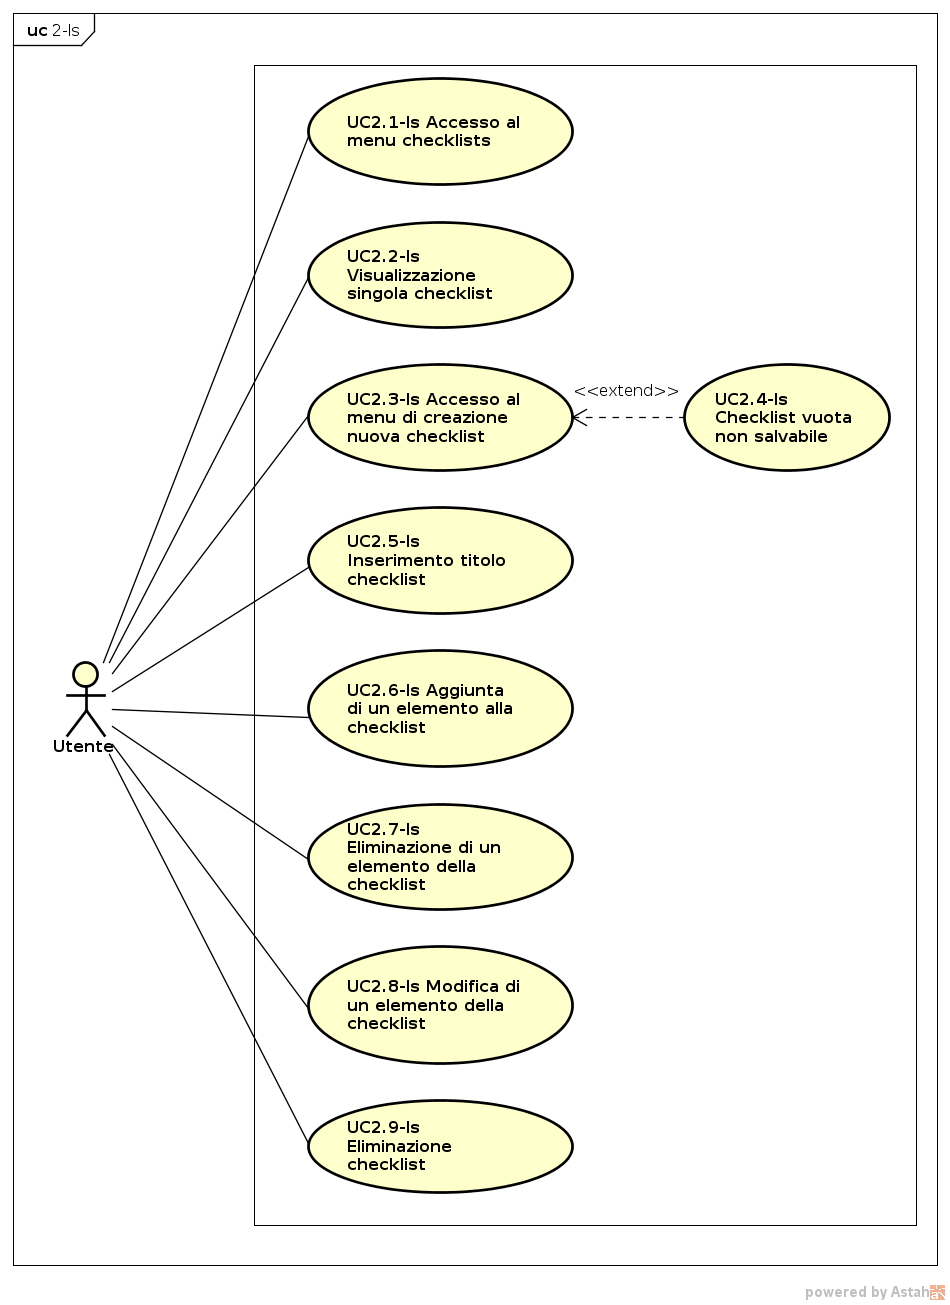
\includegraphics[scale=0.45]{img/lista2.png}
   \caption{Diagramma per il caso d'uso UC2-ls.}
\end{figure}
\FloatBarrier
\item[]\textbf{Descrizione:} Viene creata una checklist su cui basare liste future.
\item[]\textbf{Attori:} Utente. 
\item[]\textbf{Precondizione:} La bolla è utilizzabile sul sistema del mittente e in quello del ricevente. 
\item[]\textbf{Postcondizione:} Una checklist è stata creata. 
\item[]\textbf{Scenario:}
\begin{enumerate}

\item L'utente accede al menu di gestione checklists (UC2.1-ls)
\item L'utente visualizza la singola checklist (UC2.2-ls)
\item L'utente effettua l'accesso al menu di creazione di una nuova checklist (UC2.3-ls)
\item L'utente inserisce un titolo per la checklist (UC2.5-ls)
\item L'utente aggiunge un elemento alla checklist (UC2.6-ls)
\item L'utente elimina un elemento della checklist (UC2.7-ls)
\item L'utente modifica un elemento della checklist (UC2.8-ls)
\item L'utente elimina una checklist (UC2.9-ls)

\end{enumerate} 
\end{itemize}

\subsection{Caso d'uso UC2.1-ls: Accesso al menu checklists.}
\begin{itemize}
\item[]\textbf{Descrizione:} Viene effettuato l'accesso al menu di gestione delle checklists.
\item[]\textbf{Attori:} Utente. 
\item[]\textbf{Precondizione:} La bolla è utilizzabile sul sistema del mittente e su quello del ricevente. 
\item[]\textbf{Postcondizione:} \'E stato effettuato l'accesso al menu di gestione delle checklist. 
\item[]\textbf{Scenario:}
L'utente effettua l'accesso al menu di gestione delle checklist 
\end{itemize}

\subsection{Caso d'uso UC2.2-ls: Visualizzazione singola checklist.}
\begin{itemize}
\item[]\textbf{Descrizione:} Viene visualizzata la singola checklist.
\item[]\textbf{Attori:} Utente. 
\item[]\textbf{Precondizione:} \'E stato effettuato l'accesso al menu di gestione delle checklists. 
\item[]\textbf{Postcondizione:} \'E stata visualizzata la singola checklist. 
\item[]\textbf{Scenario:}
L'utente visualizza la singola checklist 
\end{itemize}

\subsection{Caso d'uso UC2.3-ls: Accesso al menu di creazione nuova checklist.}
\begin{itemize}
\item[]\textbf{Descrizione:} Viene effettuato l'accesso al menu di creazione di una nuova checklist.
\item[]\textbf{Attori:} Utente. 
\item[]\textbf{Precondizione:} \'E stato effettuato l'accesso al menu di configurazione delle checklists (UC2.1-ls). 
\item[]\textbf{Postcondizione:} \'E stata effettuato l'accesso al menu di creazione di una nuova checklist. 
\item[]\textbf{Scenario:}
L'utente effettua l'accesso al menu di creazione di una nuova checklist 
\item[]\textbf{Estensioni:}
Nel caso in cui la nuova checklist rimanga vuota, questa non verrà salvata (UC2.4-ls) 
\end{itemize}

\subsection{Caso d'uso UC2.4-ls: Checklist vuota non salvabile.}
\begin{itemize}
\item[]\textbf{Descrizione:} Nel caso in cui una nuova checklist venga lasciata vuota, questa non verrà salvata.
\item[]\textbf{Attori:} Utente. 
\item[]\textbf{Precondizione:} Si è iniziato a creare una nuova checklist. 
\item[]\textbf{Postcondizione:} La nuova checklist vuota non è stata salvata. 
\item[]\textbf{Scenario:}
L'utente ha lasciato la nuova checklist vuota e questa non è stata salvata 
\end{itemize}

\subsection{Caso d'uso UC2.5-ls: Inserimento titolo checklist.}
\begin{itemize}
\item[]\textbf{Descrizione:} Viene inserito un titolo per la nuova checklist.
\item[]\textbf{Attori:} Utente. 
\item[]\textbf{Precondizione:} \'E stato visualizzato il menu di configurazione della nuova checklist (UC2.3-ls). 
\item[]\textbf{Postcondizione:} \'E stato inserito un titolo per la checklist. 
\item[]\textbf{Scenario:}
L'utente inserisce un titolo per la checklist 
\end{itemize}

\subsection{Caso d'uso UC2.6-ls: Aggiunta di un elemento alla checklist.}
\begin{itemize}
\item[]\textbf{Descrizione:} Viene aggiunto un elemento alla checklist.
\item[]\textbf{Attori:} Utente. 
\item[]\textbf{Precondizione:} \'E stato effettuato l'accesso al menu di creazione di una nuova checklist (UC2.3-ls) oppure è stata visualizzata una checklist esistente (UC2.2-ls). 
\item[]\textbf{Postcondizione:} \'E stato aggiunto un elemento alla checklist. 
\item[]\textbf{Scenario:}
L'utente aggiunge un elemento alla checklist 
\end{itemize}

\subsection{Caso d'uso UC2.7-ls: Eliminazione di un elemento della checklist.}
\begin{itemize}
\item[]\textbf{Descrizione:} Viene eliminato un elemento della checklist.
\item[]\textbf{Attori:} Utente. 
\item[]\textbf{Precondizione:} \'E stato inserito almeno un elemento nella checklist (UC2.6-ls) che è stata visualizzata (UC2.2-ls) o che si sta creando (UC2.3-ls). 
\item[]\textbf{Postcondizione:} \'E stato eliminato un elemento dalla checklist. 
\item[]\textbf{Scenario:}
L'utente elimina un elemento dalla checklist 
\end{itemize}

\subsection{Caso d'uso UC2.8-ls: Modifica di un elemento della checklist.}
\begin{itemize}
\item[]\textbf{Descrizione:} Viene modificato un elemento della checklist.
\item[]\textbf{Attori:} Utente. 
\item[]\textbf{Precondizione:} \'E stato inserito almeno un elemento nella checklist (UC2.6-ls) che è stata visualizzata (UC2.2-ls) o che si sta creando (UC2.3-ls). 
\item[]\textbf{Postcondizione:} \'E stato modificato un elemento della checklist. 
\item[]\textbf{Scenario:}
L'utente modifica un elemento della checklist 
\end{itemize}

\subsection{Caso d'uso UC2.9-ls: Eliminazione checklist.}
\begin{itemize}
\item[]\textbf{Descrizione:} Viene eliminata una checklist.
\item[]\textbf{Attori:} Utente. 
\item[]\textbf{Precondizione:} \'E stata creata almeno una checklist (UC2.3-ls) e è stato effettuato l'accesso al menu di configurazione delle checklists (UC2.1-ls). 
\item[]\textbf{Postcondizione:} \'E stata eliminata una checklist. 
\item[]\textbf{Scenario:}
L'utente elimina una checklist 
\end{itemize}

\subsection{Caso d'uso UC3-ls: Spunta della voce.}
\begin{itemize}
\item[]\textbf{Descrizione:} Viene spuntata una voce dalla lista ricevuta.
\item[]\textbf{Attori:} Ricevente. 
\item[]\textbf{Precondizione:} L'utente ha composto e inviato una lista. 
\item[]\textbf{Postcondizione:} Una voce è stata spuntata. 
\item[]\textbf{Scenario:}
Il ricevente spunta una voce dalla lista inviatagli. 
\end{itemize}

\subsection{Caso d'uso UC4-ls: Visualizzazione delle spunte.}
\begin{itemize}
\item[]\textbf{Descrizione:} Vengono visualizzate le spunte effettuate sugli elementi della lista.
\item[]\textbf{Attori:} Utente. 
\item[]\textbf{Precondizione:} La lista è stata inviata (UC6-ls). 
\item[]\textbf{Postcondizione:} Sono state visualizzate le spunte. 
\item[]\textbf{Scenario:}
L'utente o il ricevente visualizzano le spunte effettuate sugli elementi della lista. 
\end{itemize}

\subsection{Caso d'uso UC5-ls: Visualizzazione menu di configurazione.}
\begin{itemize}
\item[]\textbf{Descrizione:} Viene visualizzato il menu di configurazione della bolla lista.
\item[]\textbf{Attori:} Utente. 
\item[]\textbf{Precondizione:} La bolla è utilizzabile sul sistema del mittente e su quello del ricevente. 
\item[]\textbf{Postcondizione:} \'E stato visualizzato il menu di configurazione della bolla. 
\item[]\textbf{Scenario:}
L'utente visualizza il menu di configurazione della bolla 
\end{itemize}

\subsection{Caso d'uso UC6-ls: Invio bolla.}
\begin{itemize}
\item[]\textbf{Descrizione:} La bolla viene inviata.
\item[]\textbf{Attori:} Utente. 
\item[]\textbf{Precondizione:} \'E stata definita una lista non vuota da inviare (UC1-ls). 
\item[]\textbf{Postcondizione:} La bolla è stata inviata. 
\item[]\textbf{Scenario:}
L'utente invia la bolla lista 
\end{itemize}

\clearpage

\subsection{Caso d'uso UC0-mt: Meteo.}
\begin{itemize}
   \FloatBarrier
   \begin{figure}[ht]
   \centering
   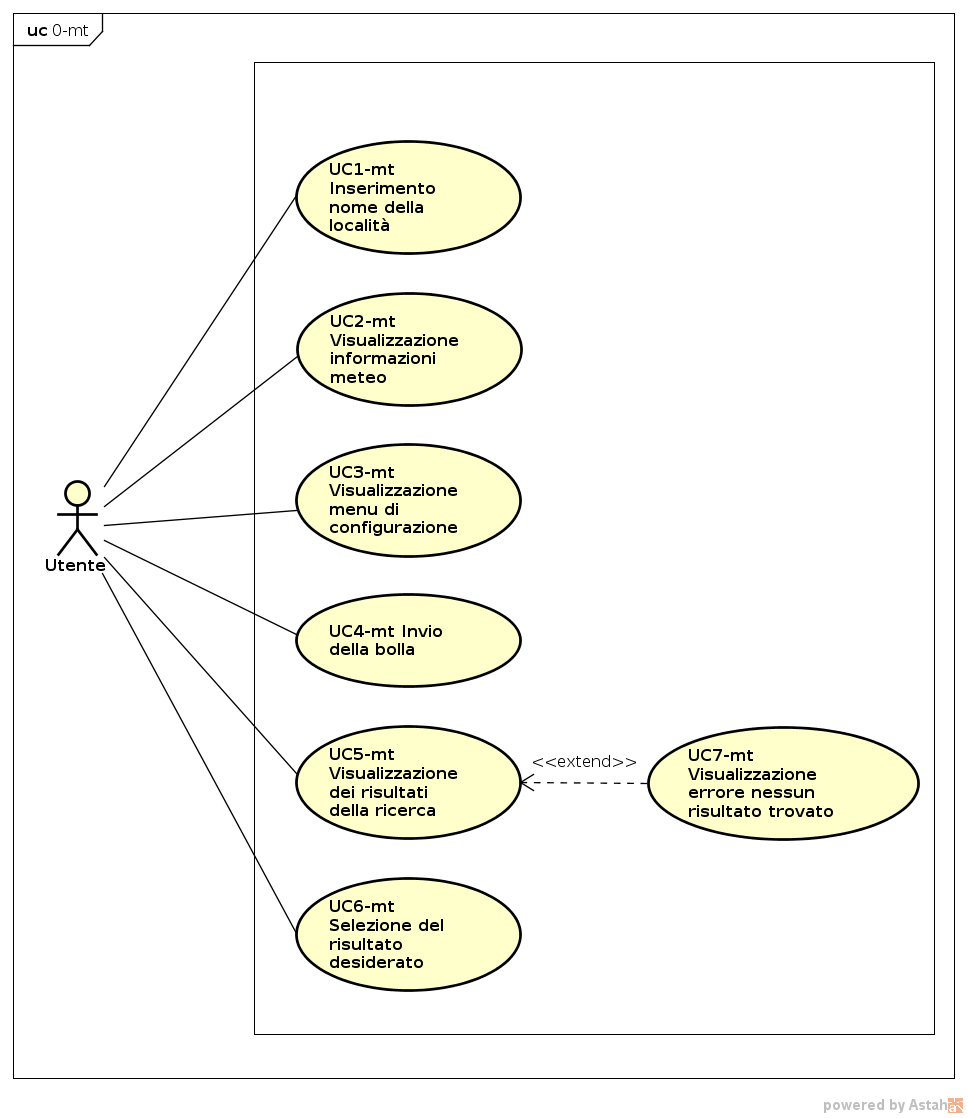
\includegraphics[scale=0.45]{img/meteo.png}
   \caption{Diagramma per il caso d'uso UC0-mt.}
\end{figure}
\FloatBarrier
\item[]\textbf{Descrizione:} La bolla restituisce le previsioni meteo per la località scelta.
\item[]\textbf{Attori:} Utente. 
\item[]\textbf{Precondizione:} La bolla è utilizzabile sul sistema del mittente e del ricevente. 
\item[]\textbf{Postcondizione:} La bolla mostra le previsioni meteo per la località scelta. 
\item[]\textbf{Scenario:}
\begin{enumerate}



\item L'utente inserisce il nome di una località (UC1-mt)

\item L'utente visualizza le informazioni meteorologiche per la località selezionata (UC2-mt)

\item L'utente visualizza il menu di configurazione della bolla (UC3-mt)
\item L'utente invia la bolla (UC4-mt)

\item L'utente visualizza i risultati della ricerca (UC5-mt)
\item L'utente seleziona il risultato desiderato tra quelli proposti (UC6-mt)



\end{enumerate} 
\end{itemize}

\subsection{Caso d'uso UC1-mt: Inserimento nome della località.}
\begin{itemize}
\item[]\textbf{Descrizione:} Viene inserito il nome della località di cui si desidera visualizzare il meteo.
\item[]\textbf{Attori:} Utente. 
\item[]\textbf{Precondizione:} \'E stato visualizzato il menu di configurazione (UC3-mt). 
\item[]\textbf{Postcondizione:} L'utente ha inserito il nome della località desiderata. 
\item[]\textbf{Scenario:}
L'utente seleziona la località desiderata. 
\end{itemize}

\subsection{Caso d'uso UC2-mt: Visualizzazione informazioni meteo.}
\begin{itemize}
\item[]\textbf{Descrizione:} Vengono visualizzate le informazioni meteorologiche richieste.
\item[]\textbf{Attori:} Utente. 
\item[]\textbf{Precondizione:} L'utente ha inviato la bolla (UC4-mt). 
\item[]\textbf{Postcondizione:} Le informazioni relative alle previsioni meteo sono state visualizzate. 
\item[]\textbf{Scenario:}
L'utente visualizza le informazioni meteorologiche richieste. 
\end{itemize}

\subsection{Caso d'uso UC3-mt: Visualizzazione menu di configurazione.}
\begin{itemize}
\item[]\textbf{Descrizione:} Viene visualizzato il menu di configurazione della bolla.
\item[]\textbf{Attori:} Utente. 
\item[]\textbf{Precondizione:} La bolla è utilizzabile sul sistema del mittente e del ricevente. 
\item[]\textbf{Postcondizione:} \'E stato visualizzato il menu di configurazione. 
\item[]\textbf{Scenario:}
L'utente visualizza il menu di configurazione per la bolla meteo 
\end{itemize}

\subsection{Caso d'uso UC4-mt: Invio della bolla.}
\begin{itemize}
\item[]\textbf{Descrizione:} La bolla viene inviata.
\item[]\textbf{Attori:} Utente. 
\item[]\textbf{Precondizione:} \'E stata selezionata la località di cui si desidera il meteo tra i risultati della ricerca (UC6-mt). 
\item[]\textbf{Postcondizione:} La bolla meteo è stata inviata. 
\item[]\textbf{Scenario:}
L'utente invia la bolla meteo 
\end{itemize}

\subsection{Caso d'uso UC5-mt: Visualizzazione dei risultati della ricerca.}
\begin{itemize}
\item[]\textbf{Descrizione:} Vengono visualizzati tutti i risultati della ricerca effettuata utilizzando il nome della località fornito.
\item[]\textbf{Attori:} Utente. 
\item[]\textbf{Precondizione:} \'E stato inserito il nome della località di cui cercare il meteo (UC1-mt). 
\item[]\textbf{Postcondizione:} Sono stati visualizzati i risultati della ricerca. 
\item[]\textbf{Scenario:}
L'utente visualizza i risultati della ricerca effettuata utilizzando il nome della località fornito 
\item[]\textbf{Estensioni:}
Nel caso in cui la ricerca non fornisca risultati viene visualizzato un messaggio di errore (UC7-mt) 
\end{itemize}

\subsection{Caso d'uso UC6-mt: Selezione del risultato desiderato.}
\begin{itemize}
\item[]\textbf{Descrizione:} Viene selezionato uno tra i risultati della ricerca.
\item[]\textbf{Attori:} Utente. 
\item[]\textbf{Precondizione:} Sono stati mostrati i risultati della ricerca (UC5-mt). 
\item[]\textbf{Postcondizione:} \'E stato selezionato uno dei risultati. 
\item[]\textbf{Scenario:}
L'utente seleziona uno tra i risultati della ricerca 
\end{itemize}

\subsection{Caso d'uso UC7-mt: Visualizzazione errore nessun risultato trovato.}
\begin{itemize}
\item[]\textbf{Descrizione:} Viene visualizzato un messaggio di errore che spiega che la ricerca effettuata utilizzando il nome della località fornito non ha prodotto alcun esito.
\item[]\textbf{Attori:} Utente. 
\item[]\textbf{Precondizione:} \'E stato inserito il nome della località di cui cercare il meteo. 
\item[]\textbf{Postcondizione:} \'E stato visualizzato il messaggio di errore. 
\item[]\textbf{Scenario:}
L'utente visualizza un messaggio di errore che spiega che la ricerca effettuata utilizzando il nome della località fornito non ha prodotto alcun esito. 
\end{itemize}

\clearpage

\subsection{Caso d'uso UC0-sd: Sondaggio.}
\begin{itemize}
   \FloatBarrier
   \begin{figure}[ht]
   \centering
   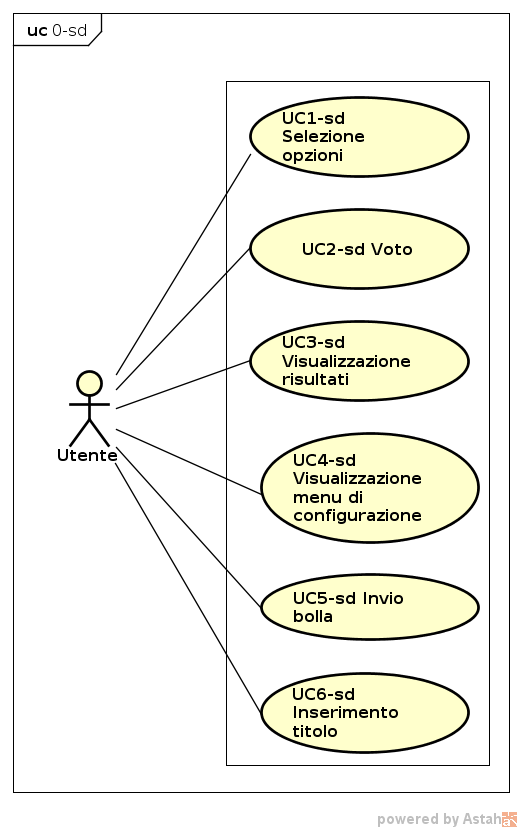
\includegraphics[scale=0.45]{img/sondaggio.png}
   \caption{Diagramma per il caso d'uso UC0-sd.}
\end{figure}
\FloatBarrier
\item[]\textbf{Descrizione:} L'utente seleziona un certo numero di opzioni tra cui i riceventi possono scegliere.
\item[]\textbf{Attori:} Utente. 
\item[]\textbf{Precondizione:} La bolla è utilizzabile sul sistema del mittente e del ricevente. 
\item[]\textbf{Postcondizione:} Il sondaggio si è concluso. 
\item[]\textbf{Scenario:}
\begin{enumerate}



\item L'utente seleziona le opzioni tra cui è possibile scegliere (UC1-sd).


\item L'utente sceglie un'opzione da votare (UC2-sd)
\item L'utente visualizza i risultati (UC3-sd)
\item L'utente visualizza il menu di configurazione della bolla (UC4-sd)
\item L'utente invia la bolla (UC5-sd)
\item L'utente inserisce il titolo (UC6-sd)
\end{enumerate} 
\end{itemize}

\subsection{Caso d'uso UC1-sd: Seleziona opzioni.}
\begin{itemize}
\item[]\textbf{Descrizione:} Vengono impostate le opzioni di voto.
\item[]\textbf{Attori:} Utente. 
\item[]\textbf{Precondizione:} \'E stato visualizzato il menu di configurazione (UC4-sd). 
\item[]\textbf{Postcondizione:} La bolla è stata impostata con i parametri del sondaggio. 
\item[]\textbf{Scenario:}
L'utente imposta le opzioni di voto. 
\end{itemize}

\subsection{Caso d'uso UC2-sd: Voto.}
\begin{itemize}
\item[]\textbf{Descrizione:} Vengono espresse le preferenze sulle opzioni proposte.
\item[]\textbf{Attori:} Utente. 
\item[]\textbf{Precondizione:} La bolla è stata inviata (UC5-sd). 
\item[]\textbf{Postcondizione:} L'utente ha espresso il voto. 
\item[]\textbf{Scenario:}
L'utente esprime una preferenza tra le opzioni proposte. 
\end{itemize}

\subsection{Caso d'uso UC3-sd: Visualizzazione risultati.}
\begin{itemize}
\item[]\textbf{Descrizione:} Vengono visualizzati i risultati della consultazione.
\item[]\textbf{Attori:} Utente. 
\item[]\textbf{Precondizione:} La bolla è stata inviata (UC5-sd). 
\item[]\textbf{Postcondizione:} I risultati sono stati visualizzati. 
\item[]\textbf{Scenario:}
L'utente e i riceventi visualizzano i risultati 
\end{itemize}

\subsection{Caso d'uso UC4-sd: Visualizzazione del menu di configurazione.}
\begin{itemize}
\item[]\textbf{Descrizione:} Viene visualizzato il menu di configurazione per la bolla sondaggio.
\item[]\textbf{Attori:} Utente. 
\item[]\textbf{Precondizione:} La bolla è utilizzabile sia sul sistema del mittente che in quello del ricevente. 
\item[]\textbf{Postcondizione:} \'E stato visualizzato il menu di configurazione. 
\item[]\textbf{Scenario:}
L'utente visualizza il menu di configurazione per la bolla sondaggio 
\end{itemize}

\subsection{Caso d'uso UC5-sd: Invio della bolla.}
\begin{itemize}
\item[]\textbf{Descrizione:} La bolla sondaggio viene inviata.
\item[]\textbf{Attori:} Utente. 
\item[]\textbf{Precondizione:} Devono essere state selezionate le opzioni di voto (UC1-sd) e il titolo (UC6-sd). 
\item[]\textbf{Postcondizione:} La bolla è stata inviata. 
\item[]\textbf{Scenario:}
L'utente invia la bolla sondaggio 
\end{itemize}

\subsection{Caso d'uso UC6-sd: Inserimento titolo.}
\begin{itemize}
\item[]\textbf{Descrizione:} Viene inserito il titolo del sondaggio.
\item[]\textbf{Attori:} Utente. 
\item[]\textbf{Precondizione:} \'E stato visualizzato il menu di configurazione (UC4-sd). 
\item[]\textbf{Postcondizione:} \'E stato inserito il titolo per il sondaggio. 
\item[]\textbf{Scenario:}
L'utente inserisce il titolo per il sondaggio 
\end{itemize}

\clearpage

\subsection{Caso d'uso UC0-tr: Bolla traduttore automatico.}
\begin{itemize}
   \FloatBarrier
   \begin{figure}[ht]
   \centering
   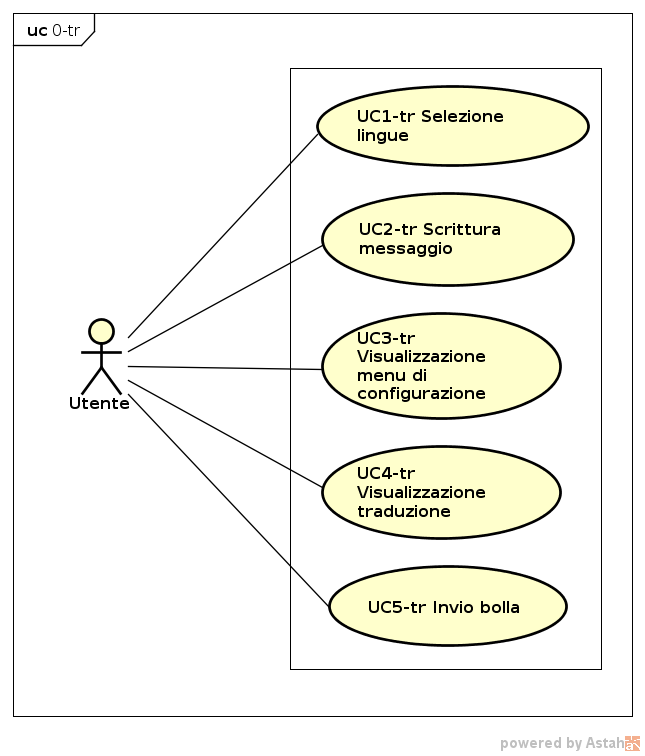
\includegraphics[scale=0.45]{img/traduttore.png}
   \caption{Diagramma per il caso d'uso UC0-tr.}
\end{figure}
\FloatBarrier
\item[]\textbf{Descrizione:} Una bolla che trade il testo inserito nelle lingue selezionate.
\item[]\textbf{Attori:} Utente. 
\item[]\textbf{Precondizione:} La bolla è utilizzabile sul sistema del mittente e del ricevente. 
\item[]\textbf{Postcondizione:} Il messaggio viene visualizzato tradotto nella lingua obiettivo. 
\item[]\textbf{Scenario:}
\begin{enumerate}



\item L'utente seleziona le lingue di partenza e d'arrivo(1-tr). 

\item L'utente scrive il messaggio (UC2-tr)

\item L'utente visualizza il menu di configurazione della bolla (UC3-tr)

\item L'utente visualizza la traduzione(4-tr)

\item L'utente invia la bolla (UC5-tr)
\end{enumerate} 
\end{itemize}

\subsection{Caso d'uso UC1-tr: Selezione della lingua di partenza.}
\begin{itemize}
\item[]\textbf{Descrizione:} Viene selezionata la lingua di partenza.
\item[]\textbf{Attori:} Utente. 
\item[]\textbf{Precondizione:} Il menu di configurazione è stato visualizzato (UC3-tr). 
\item[]\textbf{Postcondizione:} La bolla è configurata con una lingua di partenza e una d'arrivo. 
\item[]\textbf{Scenario:}
L'utente seleziona la lingua in cui sarà scritto il messaggio e quella in cui dovrà essere tradotto 
\end{itemize}

\subsection{Caso d'uso UC2-tr: Scrittura del messaggio.}
\begin{itemize}
\item[]\textbf{Descrizione:} Viene inserito il testo del messaggio da tradurre.
\item[]\textbf{Attori:} Utente. 
\item[]\textbf{Precondizione:} Il menu di configurazione è stato visualizzato (UC3-tr). 
\item[]\textbf{Postcondizione:} Il testo del messaggio è stato inserito. 
\item[]\textbf{Scenario:}
L'utente inserisce il testo del messaggio che deve essere tradotto. 
\end{itemize}

\subsection{Caso d'uso UC3-tr: Visualizzazione menu di configurazione.}
\begin{itemize}
\item[]\textbf{Descrizione:} Viene visualizzato il menu di configurazione per la bolla traduttore.
\item[]\textbf{Attori:} Utente. 
\item[]\textbf{Precondizione:} La bolla è utilizzabile sul sistema del mittente e su quello del ricevente. 
\item[]\textbf{Postcondizione:} \'E stato visualizzato il menu di configurazione. 
\item[]\textbf{Scenario:}
L'utente visualizza il menu di configurazione per la bolla traduttore 
\end{itemize}

\subsection{Caso d'uso UC4-tr: Visualizzazione traduzione.}
\begin{itemize}
\item[]\textbf{Descrizione:} Viene visualizzata la traduzione nella lingua scelta.
\item[]\textbf{Attori:} Utente. 
\item[]\textbf{Precondizione:} La bolla è stata inviata (UC5-tr). 
\item[]\textbf{Postcondizione:} \'E stato visualizzato il testo tradotto nella lingua scelta. 
\item[]\textbf{Scenario:}
L'utente e il ricevente visualizzano la traduzione 
\end{itemize}

\subsection{Caso d'uso UC5-tr: Invio bolla.}
\begin{itemize}
\item[]\textbf{Descrizione:} La bolla viene inviata.
\item[]\textbf{Attori:} Utente. 
\item[]\textbf{Precondizione:} Sono state selezionate le lingue in ingresso e in uscita (UC1-tr) e è stato scritto il messaggio (UC2-tr). 
\item[]\textbf{Postcondizione:} La bolla è stata inviata. 
\item[]\textbf{Scenario:}
L'utente invia la bolla traduttore 
\end{itemize}


\clearpage







%%%%%%%%%%%%%%%%%%%%%%%%%%%%%%%%%%%%%%%%%%%%%%%%%%%%%%%%%%%%%%%%%%%%%%%%
\section{Requisiti}

I requisiti sono organizzati per utilità strategica:
\begin{itemize}
\item Ob: Obbligatori
\item De: Desiderabili
\item Op: Opzionali
\end{itemize}
Ogni requisito dovrà essere distinto, inoltre, in base al tipo e quindi al modo in cui dovrà essere verificato:
\begin{itemize}
\item Fu: Funzionale
\item Qu: Qualitativo
\item Di: Dichiarativo
\end{itemize}
Ogni requisito dovrà rispettare la seguente codifica:
$$
R[\text{utilità strategica}][\text{tipo}][\text{codice}]-[\text{sigla
    bolla}]
$$

Dove la sigla bolla è una parte opzionale del codice che indica una
bolla predefinita allo stesso modo dei codici degli use case.
I requisiti sono di seguito esposti suddivisi per tipo.

\subsection{Requisiti funzionali}

\begin{center}
\begin{longtable}{|
*{1}{>{\centering\arraybackslash}p{2.5cm}|}
*{1}{>{\centering\arraybackslash}p{2cm}|}
*{1}{>{\centering\arraybackslash}p{5cm}|}
*{1}{>{\centering\arraybackslash}p{2.5cm}|}}
\hline \textbf{Requisito} & \textbf{Tipologia} & \textbf{Descrizione} & \textbf{Fonti}\\
\hline \endhead
\hline \endfoot

RObFu10 & \makecell{Obbligatorio \\ Funzionale} & L'utente deve poter accedere alle bolle dall'interfaccia di Rocket.Chat. & \makecell{UC3}\\
\hline

RObFu10.1 & \makecell{Obbligatorio \\ Funzionale} & All'interfaccia standard di Rocket.Chat devono essere aggiunti due pulsanti nella tabbar laterale che permettano di accedere alle SideAreas. & \makecell{UC3.1}\\
\hline

RObFu10.2 & \makecell{Obbligatorio \\ Funzionale} & L'utente deve poter utilizzare la SideArea1 che permette di creare, inviare, visualizzare e modificare le bolle inviate. & \makecell{UC3.2}\\
\hline

RObFu10.2.1 & \makecell{Obbligatorio \\ Funzionale} & L'utente deve poter visualizzare i tipi di bolla disponibili. & \makecell{UC3.2.1}\\
\hline

RObFu10.2.2 & \makecell{Obbligatorio \\ Funzionale} & L'utente deve poter selezionare il tipo di bolla da inviare. & \makecell{UC3.2.2}\\
\hline

RObFu10.2.3 & \makecell{Obbligatorio \\ Funzionale} & L'utente deve poter configurare la bolla tramite l'apposito menu. & \makecell{UC3.2.3}\\
\hline

RObFu10.2.4 & \makecell{Obbligatorio \\ Funzionale} & L'utente deve poter inviare la bolla che ha configurato. & \makecell{UC3.2.4}\\
\hline

RObFu10.2.5 & \makecell{Obbligatorio \\ Funzionale} & L'utente deve poter visualizzare lo storico delle bolle che ha inviato. & \makecell{UC3.2.5}\\
\hline

RObFu10.2.5.1 & \makecell{Obbligatorio \\ Funzionale} & L'utente deve visualizzare un messaggio appropriato nel caso non ci siano bolle nello storico in uscita. & \makecell{UC3.2.7}\\
\hline

RObFu10.2.6 & \makecell{Obbligatorio \\ Funzionale} & L'utente deve poter interagire con le bolle inviate. & \makecell{UC3.2.6}\\
\hline

RObFu10.2.7 & \makecell{Obbligatorio \\ Funzionale} & L'utente deve poter visualizzare un messaggio di errore nel caso in cui la configurazione della bolla non fosse andata a buon fine. & \makecell{UC3.2.8}\\
\hline

RObFu10.3 & \makecell{Obbligatorio \\ Funzionale} & L'utente deve poter utilizzare la SideArea2 che permette di visualizzare e interagire con le bolle ricevute. & \makecell{UC3.3}\\
\hline

RObFu10.3.1 & \makecell{Obbligatorio \\ Funzionale} & L'utente deve poter visualizzare lo storico delle bolle ricevute. & \makecell{UC3.3.1}\\
\hline

RObFu10.3.1.1 & \makecell{Obbligatorio \\ Funzionale} & L'utente deve visualizzare un messaggio appropriato nel caso in cui non ci siano bolle nello storico in ingresso. & \makecell{UC3.3.3}\\
\hline

RObFu10.3.2 & \makecell{Obbligatorio \\ Funzionale} & L'utente deve poter interagire con le bolle che ha ricevuto. & \makecell{UC3.3.2}\\
\hline

RObFu11 & \makecell{Obbligatorio \\ Funzionale} & Lo sviluppatore deve avere a disposizione gli strumenti per creare una bolla funzionante. & \makecell{UC0}\\
\hline

RObFu11.1 & \makecell{Obbligatorio \\ Funzionale} & Lo sviluppatore deve poter creare le proprie bolle a partire dalla bolla vuota. & \makecell{UC1}\\
\hline

RObFu11.2 & \makecell{Obbligatorio \\ Funzionale} & Lo sviluppatore deve poter accedere alle funzionalità offerte dall'API. & \makecell{UC2}\\
\hline

RObFu11.2.1 & \makecell{Obbligatorio \\ Funzionale} & Lo sviluppatore deve poter utilizzare le funzionalità offerte dal sistema per descrivere l'aspetto visuale delle bolle. & \makecell{UC2.1}\\
\hline

RObFu11.2.1.1 & \makecell{Obbligatorio \\ Funzionale} & Lo sviluppatore deve poter inserire un componente grafico. & \makecell{UC2.1.1}\\
\hline

RObFu11.2.1.1.1 & \makecell{Obbligatorio \\ Funzionale} & Lo sviluppatore deve poter inserire un componente testo. & \makecell{Interno\\UC2.1.1}\\
\hline

RObFu11.2.1.1.2 & \makecell{Obbligatorio \\ Funzionale} & Lo sviluppatore deve poter inserire un componente immagine. & \makecell{Interno\\UC2.1.1}\\
\hline

RObFu11.2.1.1.3 & \makecell{Obbligatorio \\ Funzionale} & Lo sviluppatore deve poter inserire un componente campo di inserimento testo. & \makecell{Interno\\UC2.1.1}\\
\hline

RObFu11.2.1.1.4 & \makecell{Obbligatorio \\ Funzionale} & Lo sviluppatore deve poter inserire un componente pulsante. & \makecell{UC2.1.1\\interno}\\
\hline

RObFu11.2.1.1.5 & \makecell{Obbligatorio \\ Funzionale} & Lo sviluppatore deve poter inserire un componente checkbox. & \makecell{Interno\\UC2.1.1}\\
\hline

RObFu11.2.1.1.6 & \makecell{Obbligatorio \\ Funzionale} & Lo sviluppatore deve poter inserire un componente radiobutton. & \makecell{Interno\\UC2.1.1}\\
\hline

RObFu11.2.1.2 & \makecell{Obbligatorio \\ Funzionale} & Lo sviluppatore deve poter inserire un contenitore. & \makecell{UC2.1.1}\\
\hline

RObFu11.2.1.2.1 & \makecell{Obbligatorio \\ Funzionale} & Lo sviluppatore deve poter inserire un contenitore che posiziona gli elementi figli uno accanto all'altro dando a ciascuno uguale spazio. Il massimo numero di elementi accostabili è 12 a causa dei limiti del grid system di Bootstap. & \makecell{Interno\\UC2.1.1}\\
\hline

RObFu11.2.1.2.2 & \makecell{Obbligatorio \\ Funzionale} & Lo sviluppatore deve poter inserire un contenitore che posiziona gli elementi figli uno sotto l'altro. & \makecell{Interno\\UC2.1.1}\\
\hline

RObFu11.2.1.2.3 & \makecell{Obbligatorio \\ Funzionale} & Lo sviluppatore deve poter inserire un contenitore il cui contenuto possa essere visualizzato o meno in base all'esecuzione di un comando. & \makecell{Interno\\UC2.1.1}\\
\hline

RObFu11.2.1.3 & \makecell{Obbligatorio \\ Funzionale} & Lo sviluppatore deve poter modificare le proprietà di un componente grafico. & \makecell{UC2.1.2}\\
\hline

RObFu11.2.1.3.1 & \makecell{Obbligatorio \\ Funzionale} & Lo sviluppatore deve poter impostare le opzioni di scelta di un radiobutton. & \makecell{UC2.1.2.6}\\
\hline

RObFu11.2.1.3.2 & \makecell{Obbligatorio \\ Funzionale} & Lo sviluppatore deve poter modificare il contenuto di un componente testo. & \makecell{UC2.1.2.1}\\
\hline

RObFu11.2.1.3.3 & \makecell{Obbligatorio \\ Funzionale} & Lo sviluppatore deve poter impostare il percorso dell'immagine da visualizzare in un componente immagine. & \makecell{UC2.1.2.2}\\
\hline

RObFu11.2.1.3.4 & \makecell{Obbligatorio \\ Funzionale} & Lo sviluppatore deve poter modificare il testo mostrato nel pulsante. & \makecell{UC2.1.2.3}\\
\hline

RObFu11.2.1.3.5 & \makecell{Obbligatorio \\ Funzionale} & Lo sviluppatore deve poter impostare l'azione da associare al pulsante. & \makecell{UC2.1.2.4}\\
\hline

RObFu11.2.1.3.6 & \makecell{Obbligatorio \\ Funzionale} & Lo sviluppatore deve poter impostare il testo della checkbox. & \makecell{UC2.1.2.5}\\
\hline

RObFu11.2.1.6 & \makecell{Obbligatorio \\ Funzionale} & Lo sviluppatore deve poter inserire il menu di configurazione della bolla. & \makecell{UC2.1.4}\\
\hline

RObFu11.2.1.7 & \makecell{Obbligatorio \\ Funzionale} & Lo sviluppatore deve poter selezionare un componente grafico o un contenitore. & \makecell{UC2.1.3}\\
\hline

RObFu11.2.2 & \makecell{Obbligatorio \\ Funzionale} & Deve essere possibile distinguere il mittente di una bolla da tutti gli altri utenti. & \makecell{UC2.2}\\
\hline

RObFu11.2.3 & \makecell{Obbligatorio \\ Funzionale} & Lo sviluppatore deve poter gestire la persistenza dei dati della bolla. & \makecell{UC2.3}\\
\hline

RObFu11.2.3.1 & \makecell{Obbligatorio \\ Funzionale} & Lo sviluppatore deve poter impostare la memorizzazione di dati nella bolla. & \makecell{Interno\\UC2.3}\\
\hline

RObFu11.2.3.2 & \makecell{Obbligatorio \\ Funzionale} & Lo sviluppatore deve poter impostare la modifica dei dati memorizzati nella bolla. & \makecell{Interno\\UC2.3}\\
\hline

RObFu11.2.3.3 & \makecell{Obbligatorio \\ Funzionale} & Lo sviluppatore deve poter impostare l'eliminazione dei dati memorizzati nella bolla. & \makecell{Interno\\UC2.3}\\
\hline

RObFu20 & \makecell{Obbligatorio \\ Funzionale} & I dati relativi alle singole istanze di bolla vengono memorizzati separatamente senza che lo sviluppatore debba operare la distinzione. & \makecell{Interno}\\
\hline

RObFu21 & \makecell{Obbligatorio \\ Funzionale} & Ogni client riceve dal data-system di Meteor solo i dati che lo riguardano, ovvero quelli di tutte le bolle presenti in rooms in cui sia presente anche l'utente. & \makecell{Interno}\\
\hline

RObFu22 & \makecell{Obbligatorio \\ Funzionale} & Deve essere possibile per lo sviluppatore effettuare dei controlli sull'input dell'utente. & \makecell{Interno}\\
\hline

RObFu22.1 & \makecell{Obbligatorio \\ Funzionale} & Lo sviluppatore deve essere in grado di effettuare controlli specifici per ciascuna situazione di input da  parte dell'utente. & \makecell{Interno}\\
\hline

RObFu23 & \makecell{Obbligatorio \\ Funzionale} & Vengono forniti allo sviluppatore una serie di componenti grafici di base. & \makecell{Interno}\\
\hline

RObFu01-cv & \makecell{Obbligatorio \\ Funzionale} & L'utente può convertire importi da una valuta all'altra. & \makecell{UC0-cv}\\
\hline

RObFu01.1-cv & \makecell{Obbligatorio \\ Funzionale} & L'utente può scegliere le valute tra cui effettuare la conversione. & \makecell{UC1-cv}\\
\hline

RObFu01.2-cv & \makecell{Obbligatorio \\ Funzionale} & L'utente può inserire l'importo da convertire. & \makecell{UC2-cv}\\
\hline

RObFu01.3-cv & \makecell{Obbligatorio \\ Funzionale} & I tassi di conversione vengono forniti tramite la libreria money.js. & \makecell{Interno}\\
\hline

RObFu01.4-cv & \makecell{Obbligatorio \\ Funzionale} & Il mittente e il ricevente devono poter visualizzare gli importi convertiti. & \makecell{UC3-cv}\\
\hline

ROpFu02-cv & \makecell{Opzionale \\ Funzionale} & L'utente può convertire importi da valori di pacchetti azionari. & \makecell{Interno}\\
\hline

RObFu01-dd & \makecell{Obbligatorio \\ Funzionale} & La bolla estrae un numero casualmente dal range impostato. & \makecell{UC0-dd}\\
\hline

RObFu01.1-dd & \makecell{Obbligatorio \\ Funzionale} & L'utente deve poter impostare il range da cui estrarre il numero casuale. & \makecell{UC1-dd}\\
\hline

RObFu01.2-dd & \makecell{Obbligatorio \\ Funzionale} & Il mittente e il ricevente devono poter visualizzare il numero casuale generato. & \makecell{UC2-dd}\\
\hline

ROpFu01.2.1-dd & \makecell{Opzionale \\ Funzionale} & Il mittente e il ricevente devono poter visualizzare il numero casuale sotto forma di immagine (per esempio le facce di uno o più dadi). & \makecell{Interno}\\
\hline

RObFu01.3-dd & \makecell{Obbligatorio \\ Funzionale} & Il sistema genera lato server un numero casuale nel range specificato utilizzando la libreria Math inclusa in Javascript. & \makecell{Interno}\\
\hline

RObFu01-ls & \makecell{Obbligatorio \\ Funzionale} & Il mittente deve poter definire una lista da inviare. & \makecell{UC1-ls}\\
\hline

RObFu01.1-ls & \makecell{Obbligatorio \\ Funzionale} & Il mittente deve poter inserire manualmente un nuovo elemento. & \makecell{UC1.1-ls}\\
\hline

RObFu01.2-ls & \makecell{Obbligatorio \\ Funzionale} & Il mittente deve poter inserire un elemento prelevandolo da una delle liste predefinite. & \makecell{UC1.2-ls}\\
\hline

RObFu02-ls & \makecell{Obbligatorio \\ Funzionale} & Il mittente deve poter definire una lista predefinita. & \makecell{UC2-ls}\\
\hline

RObFu03-ls & \makecell{Obbligatorio \\ Funzionale} & Il mittente e il ricevente devono poter spuntare una voce dalla lista inviatagli. & \makecell{UC3-ls}\\
\hline

RObFu04-ls & \makecell{Obbligatorio \\ Funzionale} & Il mittente e il ricevente devono poter visualizzare le spunte effettuate. & \makecell{UC4-ls}\\
\hline

RObFu01-mt & \makecell{Obbligatorio \\ Funzionale} & La bolla deve restituire le previsioni meteo per la località scelta. & \makecell{UC0-mt}\\
\hline

RObFu01.1-mt & \makecell{Obbligatorio \\ Funzionale} & Il mittente deve poter selezionare la località desiderata. & \makecell{UC1-mt}\\
\hline

RObFu01.2-mt & \makecell{Obbligatorio \\ Funzionale} & Le previsioni meteorologiche vengono fornite tramite la libreria weather.js. & \makecell{Interno}\\
\hline

RObFu01.3-mt & \makecell{Obbligatorio \\ Funzionale} & Il mittente e il ricevente devono poter visualizzare il meteo per la località selezionata. & \makecell{UC2-mt}\\
\hline

RObFu01-sd & \makecell{Obbligatorio \\ Funzionale} & Il mittente può definire le opzioni tra cui i riceventi possono scegliere. & \makecell{UC1-sd}\\
\hline

RObFu02-sd & \makecell{Obbligatorio \\ Funzionale} & Il ricevente deve poter votare nel sondaggio. & \makecell{UC2-sd}\\
\hline

RObFu03-sd & \makecell{Obbligatorio \\ Funzionale} & Il mittente deve poter votare nel proprio sondaggio. & \makecell{UC2-sd}\\
\hline

RObFu04-sd & \makecell{Obbligatorio \\ Funzionale} & Il mittente e il ricevente devono poter visualizzare i risultati del sondaggio. & \makecell{UC3-sd}\\
\hline

RObFu01-tr & \makecell{Obbligatorio \\ Funzionale} & La bolla deve tradurre il testo inserito nelle lingue selezionate. & \makecell{UC0-tr}\\
\hline

RObFu01.1-tr & \makecell{Obbligatorio \\ Funzionale} & Il mittente deve poter configurare la lingua in cui sarà scritto il messaggio. & \makecell{UC1-tr}\\
\hline

RObFu01.2-tr & \makecell{Obbligatorio \\ Funzionale} & Il mittente deve poter inserire il testo da tradurre. & \makecell{UC2-tr}\\
\hline

RObFu01.3-tr & \makecell{Obbligatorio \\ Funzionale} & Il mittente deve poter configurare la lingua in cui il messaggio sarà tradotto. & \makecell{UC3-tr}\\
\hline

RObFu01.4-tr & \makecell{Obbligatorio \\ Funzionale} & La traduzione deve essere fornita tramite la libreria polyglot.js. & \makecell{Interno}\\
\hline

RObFu01.5-tr & \makecell{Obbligatorio \\ Funzionale} & Il mittente e il ricevente devono poter visualizzare la traduzione. & \makecell{UC4-tr}\\
\hline

\hline
\end{longtable}
\captionof{table}{Requisiti funzionali}
\end{center}
\subsection{Requisiti qualitativi}

\begin{center}
\begin{longtable}{|
*{1}{>{\centering\arraybackslash}p{2.5cm}|}
*{1}{>{\centering\arraybackslash}p{2cm}|}
*{1}{>{\centering\arraybackslash}p{5cm}|}
*{1}{>{\centering\arraybackslash}p{2.5cm}|}}
\hline \textbf{Requisito} & \textbf{Tipologia} & \textbf{Descrizione} & \textbf{Fonti}\\
\hline \endhead
\hline \endfoot

RObQu04.1 & \makecell{Obbligatorio \\ Qualitativo} & Javascript deve essere usato secondo le Airbnb style guide. & \makecell{Capitolato}\\
\hline

RObQu06 & \makecell{Obbligatorio \\ Qualitativo} & Monolith e le bolle devono essere realizzati secondo il 12 Factors app guidelines. & \makecell{Capitolato}\\
\hline

RObQu08 & \makecell{Obbligatorio \\ Qualitativo} & Monolith deve essere corredato da un manuale in inglese. & \makecell{Capitolato}\\
\hline

RObQu08.1 & \makecell{Obbligatorio \\ Qualitativo} & Il manuale deve spiegare come installare Monolith in ambiente Rochet.Chat. & \makecell{Capitolato\\Interno}\\
\hline

RObQu15 & \makecell{Obbligatorio \\ Qualitativo} & Il framework è realizzato con uso di promise per la programmazione asincrona. & \makecell{Capitolato}\\
\hline

RObQu16 & \makecell{Obbligatorio \\ Qualitativo} & La documentazione formale standard deve essere

scritta in italiano. & \makecell{Capitolato\\Verbale-2017-03-01}\\
\hline

RObQu17 & \makecell{Obbligatorio \\ Qualitativo} & La bolla presentata come Demo deve essere documentata. & \makecell{Interno}\\
\hline

\hline
\end{longtable}
\captionof{table}{Requisiti qualitativi}
\end{center}
\subsection{Requisiti dichiarativi}

\begin{center}
\begin{longtable}{|
*{1}{>{\centering\arraybackslash}p{2.5cm}|}
*{1}{>{\centering\arraybackslash}p{2cm}|}
*{1}{>{\centering\arraybackslash}p{5cm}|}
*{1}{>{\centering\arraybackslash}p{2.5cm}|}}
\hline \textbf{Requisito} & \textbf{Tipologia} & \textbf{Descrizione} & \textbf{Fonti}\\
\hline \endhead
\hline \endfoot

RObDi01 & \makecell{Obbligatorio \\ Dichiarativo} & Monolith deve essere realizzato come pacchetto RocketChat. & \makecell{Capitolato}\\
\hline

RObDi02 & \makecell{Obbligatorio \\ Dichiarativo} & Devono essere fornite alcune bolle predefinite. & \makecell{Capitolato}\\
\hline

RObDi02.1 & \makecell{Obbligatorio \\ Dichiarativo} & Una delle bolle predefinite funge da demo al fine di dimostrare l'utilizzo delle API. & \makecell{Capitolato}\\
\hline

RObDi03 & \makecell{Obbligatorio \\ Dichiarativo} & Monolith deve includere un set di API per lo sviluppo di bolle. & \makecell{Capitolato}\\
\hline

RObDi04 & \makecell{Obbligatorio \\ Dichiarativo} & Monolith deve essere realizzato usando Javascript ES6. & \makecell{Capitolato}\\
\hline

RObDi05 & \makecell{Obbligatorio \\ Dichiarativo} & Monolith deve essere realizzato usando SCSS. & \makecell{Capitolato}\\
\hline

RObDi07 & \makecell{Obbligatorio \\ Dichiarativo} & Utilizzo del framework frontend REACT per la creazione delle interfacce. & \makecell{Capitolato}\\
\hline

RObDi07.1 & \makecell{Obbligatorio \\ Dichiarativo} & I dati dei componenti React devono essere reattivi all'interno del data-system di Meteor. & \makecell{Interno}\\
\hline

RObDi09 & \makecell{Obbligatorio \\ Dichiarativo} & La demo deve essere installabile su Heroku. & \makecell{Capitolato}\\
\hline

RObDi11.2.1.2.4 & \makecell{Obbligatorio \\ Dichiarativo} & I layout offerti dai contenitori sono realizzati utilizzando il grid system di Bootstrap. & \makecell{Interno\\UC2.1.1}\\
\hline

RObDi12 & \makecell{Obbligatorio \\ Dichiarativo} & Il codice sorgente di Monolith e delle bolle deve essere disponibile su GitHub. & \makecell{Capitolato}\\
\hline

RObDi13 & \makecell{Obbligatorio \\ Dichiarativo} & Monolith deve supportare i browser in cui è eseguibile Rocket.Chat. & \makecell{Interno}\\
\hline

RObDi14 & \makecell{Obbligatorio \\ Dichiarativo} & L'interfaccia del sistema Monolith deve essere responsive. & \makecell{Interno}\\
\hline

RObDi18 & \makecell{Obbligatorio \\ Dichiarativo} & L'utilizzo di callbacks nel codice Javascript deve essere giustificato. & \makecell{Capitolato}\\
\hline

RObDi19 & \makecell{Obbligatorio \\ Dichiarativo} & La modifica del nome delle classi HTML dei componenti è realizzata attraverso l'utility classnames. & \makecell{Interno}\\
\hline

\hline
\end{longtable}
\captionof{table}{Requisiti dichiarativi}
\end{center}
\subsection{Riepilogo requisiti}

I 102 requisiti individuati si suddividono come segue:
\begin{center}
  \centering
  \begin{tabular}{|l|c|c|c|}
    \hline
      & Funzionali & Qualitativi & Dichiarativi   \\
\hline
Obbligatori &      78     &    7     & 15       \\
\hline
Desiderabili &     0     &     0     & 0    \\
\hline
Opzionali   &      2     &    0     & 0    \\
\hline
  \end{tabular}
  \captionof{table}{Riepilogo del numero di requisiti individuati.}
\end{center}


\subsection{Tracciamento fonti - requisiti per l'SDK}
\begin{center}
\begin{longtable}{|
*{1}{>{\centering\arraybackslash}p{5cm}|}
*{1}{>{\centering\arraybackslash}p{5cm}|}}
\hline \textbf{Fonte} & \textbf{Requisiti}\\
\hline \endhead
\hline \endfoot

UC0 & \makecell{RObFu11
}\\\hline
UC1 & \makecell{RObFu11.1
}\\\hline
UC2 & \makecell{RObFu11.2
}\\\hline
UC2.1 & \makecell{RObFu11.2.1
}\\\hline
UC2.1.1 & \makecell{RObFu11.2.1.1
\\RObFu11.2.1.1.1
\\RObFu11.2.1.1.2
\\RObFu11.2.1.1.3
\\RObFu11.2.1.1.4
\\RObFu11.2.1.1.5
\\RObFu11.2.1.1.6
\\RObFu11.2.1.2
\\RObFu11.2.1.2.1
\\RObFu11.2.1.2.2
\\RObFu11.2.1.2.3
\\RObDi11.2.1.2.4
}\\\hline
UC2.1.2 & \makecell{RObFu11.2.1.3
}\\\hline
UC2.1.2.1 & \makecell{RObFu11.2.1.3.2
}\\\hline
UC2.1.2.2 & \makecell{RObFu11.2.1.3.3
}\\\hline
UC2.1.2.3 & \makecell{RObFu11.2.1.3.4
}\\\hline
UC2.1.2.4 & \makecell{RObFu11.2.1.3.5
}\\\hline
UC2.1.2.5 & \makecell{RObFu11.2.1.3.6
}\\\hline
UC2.1.2.6 & \makecell{RObFu11.2.1.3.1
}\\\hline
UC2.1.3 & \makecell{RObFu11.2.1.7
}\\\hline
UC2.1.4 & \makecell{RObFu11.2.1.6
}\\\hline
UC2.2 & \makecell{RObFu11.2.2
}\\\hline
UC2.3 & \makecell{RObFu11.2.3
\\RObFu11.2.3.1
\\RObFu11.2.3.2
\\RObFu11.2.3.3
}\\\hline
UC3 & \makecell{RObFu10
}\\\hline
UC3.1 & \makecell{RObFu10.1
}\\\hline
UC3.2 & \makecell{RObFu10.2
}\\\hline
UC3.2.1 & \makecell{RObFu10.2.1
}\\\hline
UC3.2.2 & \makecell{RObFu10.2.2
}\\\hline
UC3.2.3 & \makecell{RObFu10.2.3
}\\\hline
UC3.2.4 & \makecell{RObFu10.2.4
}\\\hline
UC3.2.5 & \makecell{RObFu10.2.5
}\\\hline
UC3.2.6 & \makecell{RObFu10.2.6
}\\\hline
UC3.2.7 & \makecell{RObFu10.2.5.1
}\\\hline
UC3.2.8 & \makecell{RObFu10.2.7
}\\\hline
UC3.3 & \makecell{RObFu10.3
}\\\hline
UC3.3.1 & \makecell{RObFu10.3.1
}\\\hline
UC3.3.2 & \makecell{RObFu10.3.2
}\\\hline
UC3.3.3 & \makecell{RObFu10.3.1.1
}\\\hline
Capitolato & \makecell{RObDi01
\\RObDi02
\\RObDi02.1
\\RObDi03
\\RObDi04
\\RObQu04.1
\\RObDi05
\\RObQu06
\\RObDi07
\\RObQu08
\\RObQu08.1
\\RObDi09
\\RObDi12
\\RObQu15
\\RObQu16
\\RObDi18
}\\\hline
Interno & \makecell{RObDi07.1
\\RObQu08.1
\\RObFu11.2.1.1.1
\\RObFu11.2.1.1.2
\\RObFu11.2.1.1.3
\\RObFu11.2.1.1.4
\\RObFu11.2.1.1.5
\\RObFu11.2.1.1.6
\\RObFu11.2.1.2.1
\\RObFu11.2.1.2.2
\\RObFu11.2.1.2.3
\\RObDi11.2.1.2.4
\\RObFu11.2.3.1
\\RObFu11.2.3.2
\\RObFu11.2.3.3
\\RObDi13
\\RObDi14
\\RObQu17
\\RObDi19
\\RObFu20
\\RObFu21
\\RObFu22
\\RObFu22.1
\\RObFu23
}\\\hline
UCVerbale-2017-03-01 & \makecell{RObQu16
}\\\hline
\end{longtable}
\end{center}
\subsection{Tracciamento fonti - requisiti per le bolle}
\begin{center}
\begin{longtable}{|
*{1}{>{\centering\arraybackslash}p{5cm}|}
*{1}{>{\centering\arraybackslash}p{5cm}|}}
\hline \textbf{Fonte} & \textbf{Requisiti}\\
\hline \endhead
\hline \endfoot

UC0-cv & \makecell{RObFu01-cv
}\\\hline
UC0-dd & \makecell{RObFu01-dd
}\\\hline
UC0-mt & \makecell{RObFu01-mt
}\\\hline
UC0-tr & \makecell{RObFu01-tr
}\\\hline
UC1-cv & \makecell{RObFu01.1-cv
}\\\hline
UC1-dd & \makecell{RObFu01.1-dd
}\\\hline
UC1-ls & \makecell{RObFu01-ls
}\\\hline
UC1-mt & \makecell{RObFu01.1-mt
}\\\hline
UC1-sd & \makecell{RObFu01-sd
}\\\hline
UC1-tr & \makecell{RObFu01.1-tr
}\\\hline
UC1.1-ls & \makecell{RObFu01.1-ls
}\\\hline
UC1.2-ls & \makecell{RObFu01.2-ls
}\\\hline
UC2-cv & \makecell{RObFu01.2-cv
}\\\hline
UC2-dd & \makecell{RObFu01.2-dd
}\\\hline
UC2-ls & \makecell{RObFu02-ls
}\\\hline
UC2-mt & \makecell{RObFu01.3-mt
}\\\hline
UC2-sd & \makecell{RObFu02-sd
\\RObFu03-sd
}\\\hline
UC2-tr & \makecell{RObFu01.2-tr
}\\\hline
UC3-cv & \makecell{RObFu01.4-cv
}\\\hline
UC3-ls & \makecell{RObFu03-ls
}\\\hline
UC3-sd & \makecell{RObFu04-sd
}\\\hline
UC3-tr & \makecell{RObFu01.3-tr
}\\\hline
UC4-ls & \makecell{RObFu04-ls
}\\\hline
UC4-tr & \makecell{RObFu01.5-tr
}\\\hline
Interno & \makecell{RObFu01.2-mt
\\ROpFu01.2.1-dd
\\RObFu01.3-cv
\\RObFu01.3-dd
\\RObFu01.4-tr
\\ROpFu02-cv
}\\\hline
\end{longtable}
\end{center}

